\documentclass[]{article}
\usepackage{lmodern}
\usepackage{amssymb,amsmath}
\usepackage{ifxetex,ifluatex}
\usepackage{fixltx2e} % provides \textsubscript
\ifnum 0\ifxetex 1\fi\ifluatex 1\fi=0 % if pdftex
  \usepackage[T1]{fontenc}
  \usepackage[utf8]{inputenc}
\else % if luatex or xelatex
  \ifxetex
    \usepackage{mathspec}
  \else
    \usepackage{fontspec}
  \fi
  \defaultfontfeatures{Ligatures=TeX,Scale=MatchLowercase}
\fi
% use upquote if available, for straight quotes in verbatim environments
\IfFileExists{upquote.sty}{\usepackage{upquote}}{}
% use microtype if available
\IfFileExists{microtype.sty}{%
\usepackage{microtype}
\UseMicrotypeSet[protrusion]{basicmath} % disable protrusion for tt fonts
}{}
\usepackage[margin=1in]{geometry}
\usepackage{hyperref}
\hypersetup{unicode=true,
            pdftitle={Economic Value of Pacific Herring in the Strait of Georgia},
            pdfauthor={Tim Cashion},
            pdfborder={0 0 0},
            breaklinks=true}
\urlstyle{same}  % don't use monospace font for urls
\usepackage{longtable,booktabs}
\usepackage{graphicx,grffile}
\makeatletter
\def\maxwidth{\ifdim\Gin@nat@width>\linewidth\linewidth\else\Gin@nat@width\fi}
\def\maxheight{\ifdim\Gin@nat@height>\textheight\textheight\else\Gin@nat@height\fi}
\makeatother
% Scale images if necessary, so that they will not overflow the page
% margins by default, and it is still possible to overwrite the defaults
% using explicit options in \includegraphics[width, height, ...]{}
\setkeys{Gin}{width=\maxwidth,height=\maxheight,keepaspectratio}
\IfFileExists{parskip.sty}{%
\usepackage{parskip}
}{% else
\setlength{\parindent}{0pt}
\setlength{\parskip}{6pt plus 2pt minus 1pt}
}
\setlength{\emergencystretch}{3em}  % prevent overfull lines
\providecommand{\tightlist}{%
  \setlength{\itemsep}{0pt}\setlength{\parskip}{0pt}}
\setcounter{secnumdepth}{5}
% Redefines (sub)paragraphs to behave more like sections
\ifx\paragraph\undefined\else
\let\oldparagraph\paragraph
\renewcommand{\paragraph}[1]{\oldparagraph{#1}\mbox{}}
\fi
\ifx\subparagraph\undefined\else
\let\oldsubparagraph\subparagraph
\renewcommand{\subparagraph}[1]{\oldsubparagraph{#1}\mbox{}}
\fi

%%% Use protect on footnotes to avoid problems with footnotes in titles
\let\rmarkdownfootnote\footnote%
\def\footnote{\protect\rmarkdownfootnote}

%%% Change title format to be more compact
\usepackage{titling}

% Create subtitle command for use in maketitle
\newcommand{\subtitle}[1]{
  \posttitle{
    \begin{center}\large#1\end{center}
    }
}

\setlength{\droptitle}{-2em}

  \title{Economic Value of Pacific Herring in the Strait of Georgia}
    \pretitle{\vspace{\droptitle}\centering\huge}
  \posttitle{\par}
    \author{Tim Cashion}
    \preauthor{\centering\large\emph}
  \postauthor{\par}
      \predate{\centering\large\emph}
  \postdate{\par}
    \date{February 11, 2019}

\usepackage{booktabs}
\usepackage{longtable}
\usepackage{array}
\usepackage{multirow}
\usepackage[table]{xcolor}
\usepackage{wrapfig}
\usepackage{float}
\usepackage{colortbl}
\usepackage{pdflscape}
\usepackage{tabu}
\usepackage{threeparttable}
\usepackage{threeparttablex}
\usepackage[normalem]{ulem}
\usepackage{makecell}

\usepackage{amsthm}
\newtheorem{theorem}{Theorem}[section]
\newtheorem{lemma}{Lemma}[section]
\theoremstyle{definition}
\newtheorem{definition}{Definition}[section]
\newtheorem{corollary}{Corollary}[section]
\newtheorem{proposition}{Proposition}[section]
\theoremstyle{definition}
\newtheorem{example}{Example}[section]
\theoremstyle{definition}
\newtheorem{exercise}{Exercise}[section]
\theoremstyle{remark}
\newtheorem*{remark}{Remark}
\newtheorem*{solution}{Solution}
\begin{document}
\maketitle

{
\setcounter{tocdepth}{2}
\tableofcontents
}
Prepared for Pacific Wild

\begin{center}
\includegraphics[width=18.9in]{./PW Logo files/PNG (raster)/large-png-pacific-wild-logo/pw-logo-dark-transparent-bg@2x} \end{center}

\section{Executive Summary}\label{executive-summary}

The Pacific herring roe fishery is a longstanding fishery in BC, and its
epicenter is now the Strait of Georgia. Here, we investigate the
economic value of the fishery within the context of other fisheries in
the region and its history. In general, landings, overall value, and
prices have declined for the sector over the past 20 years. This is a
challenge to the BC seafood industry as the herring fishery has a
strategic importance to the fisheries and seafood processing sector of
generating work in the off-season, and the decrease in catches also
leads to decreases in employment in the processing and export sectors.
Those invested in the fishery have seen the decline in value as the
licences and lease costs have decreased substantially along with the
decline in value of the herring. Finally, we investigate the costs of
closing the fishery for the 2019 season as a proposed means of recovery
of the herring stocks and protection of species that rely upon them.

\subsection{Terms \& Notes}\label{terms-notes}

Ex-vessel value - the value of fish or seafood at its first point of
sale (i.e., the price the fishers receive) Unless otherwise stated, all
values are expressed in real 2015 dollars to account for inflation over
the time period studied. Tonnes refers to metric tonnes (1000 kilograms,
1kg = 2.2 lbs). Some reports use short tons (2000 lbs) and this was
converted to metric tonnes when necessary.

\section{Introduction}\label{introduction}

This report was prepared for Pacific Wild to evaluate the current value
of the Pacific herring (\emph{Clupea pallasii}) roe fishery in the
Strait of Georgia. The herring roe fishery has a long history in British
Columbia and is a valuable part of BC's seafood exports. This fishery
makes up the largest component of the Pacific herring fisheries in BC,
and is the most valuable aspect of the fishery. The herring fishery in
BC is composed of several segments: roe herring undertaken with purse
seines and gillnets, food and bait herring, herring spawn on kelp, and
special use herring. Each of these has their own (or several) licences
within the category that allow fishers to fish for this purpose. This
report focuses specifically on the seine and gillnet roe fishery, while
including the food and bait fishery and spawn on kelp fisheries when
important for context. We also focus on one key fishing ground for the
roe fishery, the Strait of Georgia (Figure \ref{fig:map}), where the
fishery has been especially concentrated in recent years.

\begin{figure}
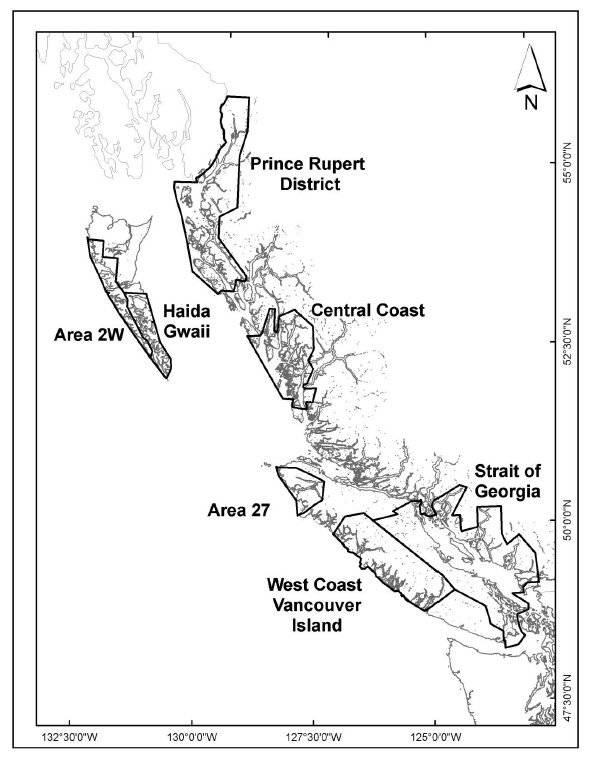
\includegraphics[width=0.5\linewidth]{DFO_Map} \caption{Figure 1. Map of roe herring fishing areas in British Columbia. Source: Fisheries and Oceans Canada, 2018.}\label{fig:map}
\end{figure}

\section{The Fisheries}\label{the-fisheries}

The Pacific herring fishery was formerly the largest fishery in BC until
the fishery collapsed in the 1960s. Until that point, most of the
fishery was used for the production of fishmeal and fish oil to support
agriculture and livestock. The fishery was re-started in the 1970s with
smaller catches destined for a high-value export of roe to the Japanese
market. This fishery has proceeded to today being the main component of
the herring fishery in BC (Figure \ref{fig:catch-by-type}), with other
fisheries being of much less importance by catch and value. The
exception to this is the spawn on kelp fishery which is fished both
commercial and as a Food, Social, and Ceremonial fishery by First
Nations in BC. The other major component of the herring fishery in BC is
the food and bait fishery. There are several other smaller special
herring fisheries that are much smaller in tonnage and value than the
three aforementioned components. Here we focus on the economically most
important fishery: the herring roe fishery (Figure
\ref{fig:roe-fishery-sog}).

\begin{figure}
\centering
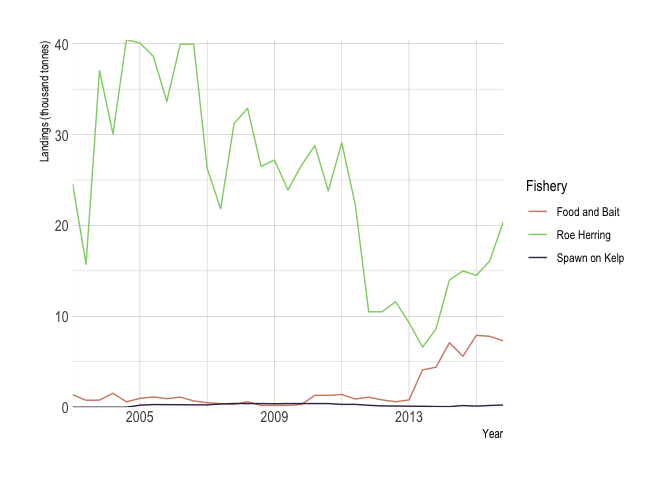
\includegraphics{index_files/figure-latex/catch-by-type-1.pdf}
\caption{\label{fig:catch-by-type}Catch of herring by fishery type. Source:
BC Ministry of Agriculture, 2018.}
\end{figure}

For the 2019 season, the expected catches across all herring fisheries
is \textasciitilde{}30,000 tonnes (Figure \ref{fig:bar-chart-area-use}).
The gillnet and seine roe fisheries are going to occur solely within the
Strait of Georgia. Outside the Strait of Georgia, there are small
fisheries as part of First Nations and commercial spawn on kelp
fisheries (SOK), as well as Food, Social, and Ceremonial (FSC)
fisheries. Other special use herring fisheries include human food and
bait, sport fishing bait, personal use and fish for zoos and aquaria
totalling \textasciitilde{}800 tonnes. Grouping these together, the only
commercial fishing outside the Strait of Georgia is for commercial spawn
on kelp herring fisheries.

\begin{figure}
\centering
\includegraphics{index_files/figure-latex/bar-chart-area-use-1.pdf}
\caption{\label{fig:bar-chart-area-use}Expected catches (metric tonnes) of
herring by area and fishery for the 2019 season areas. CC: Central
Coast; HG: Haida Gwaii; PR: Prince Rupert; SOG: Strait of Georgia; WCVI:
West Coast Vancouver Island. FSC: Food, Social, and Ceremonial; SOK:
Spawn on Kelp. Source: DFO, 2018}
\end{figure}

\begin{figure}
\centering
\includegraphics{index_files/figure-latex/roe-fishery-sog-1.pdf}
\caption{\label{fig:roe-fishery-sog}Roe herring landings by gear in the
Strait of Georgia. Source: Compiled season summary data from DFO
reports.}
\end{figure}

\section{The Products}\label{the-products}

The main product of the roe fishery is the herring roe. This is exported
in both frozen and cured forms to Japan. In general, the decline in
ex-vessel prices for herring in BC are attributed to a decline in demand
from the Japanese market. This has been attributed to a weakened
Japanese economy and a change in tastes from older to younger
generations. There is a growing share of herring products exported
outside of Japan, mainly to China and the USA (DFO 2018b).

While the roe is the backbone of the fishery, the majority by weight is
the by-product of herring carcasses used for fishmeal and fish oil.
There is limited information on the value of the carcasses, but one
processor contacted during this study said that they are not paid for
the carcasses, but they are picked up by the reduction company for no
cost. By all accounts the carcasses from the roe herring fishery are
used to produce fishmeal and fish oil in BC. This fishmeal and fish oil
are used primarily for salmon feed production that is fed to BC farmed
salmon (McGrath, Pelletier, and Tyedmers 2015). Using industry average
information, we can estimate the amount of fishmeal produced on average
from the roe herring fishery, and the amount likely required by the BC
farmed salmon industry.

The carcass weight that is used for fishmeal is between 84\% and 89\% of
the landed weight {[}McGrath, Pelletier, and Tyedmers (2015); Anonymous
Pers. Comm.{]}. The feed conversion ratio (the ratio of feed used per
output of salmon) for farmed salmon in BC was 1.313 in 2009 (Pelletier
et al. 2009). The average annual amount of farmed Atlantic salmon
produced in BC was 81,467 tonnes from 2014 to 2016 (AgriService BC
2017). A standard BC salmon feed contains 5\% herring by-product meal
and 2\% herring by-product oil (McGrath, Pelletier, and Tyedmers 2015).
Thus, we can estimate the herring fishmeal required to be 4,481 tonnes.
Alternatively, we can estimate the amount of herring fishmeal and fish
oil produced from the roe fishery by-products (averaged for 2014 and
2015) as 2,452 and 645 tonnes, respectively. Based on current export
prices for herring meal and herring oil from Canada (FAO 2016), the
value of these combined products is estimated to be 8.6 million CAD.

\section{The Supply Chain}\label{the-supply-chain}

Here, we measure employment in full-time equivalents (FTEs) to
standardize the importance of these various industries that are seasonal
by nature. A standard measure of full-time equivalent is 2080 hours
annual, defined as 40 hours per week for 52 weeks per year.

The combined fisheries for herring roe and food and bait generated 790
jobs during the season equivalent to 91 full-time equivalents
(GSGislason \& Associates Ltd. 2015). The processing of herring
generates more jobs, hours of work and total income for those involved
than the capture portion of the fishery. There are additional jobs
generated through spin-off employment including transportation,
unloading of herring, and marketing and sales, although these are a much
smaller portion when compared to fishing and processing.

\begin{figure}
\centering
\includegraphics{index_files/figure-latex/ftes-processing-1.pdf}
\caption{\label{fig:ftes-processing}Processing employment by fishery type.
Source: Estimated based on processing requirements in DFO, 2018.}
\end{figure}

\begin{figure}
\centering
\includegraphics{index_files/figure-latex/income-processing-1.pdf}
\caption{\label{fig:income-processing}Wage income from processing (inflation
adjusted million \$). Source: Estimated based on processing requirements
in DFO, 2018.}
\end{figure}

\begin{table}

\caption{\label{tab:supply-chain-table}Fishery expenses, wages, and jobs for the herring supply chain}
\centering
\begin{tabular}[t]{l|r|r|r|r|l|l}
\hline
Category & Roe expenses (\$000s) & Food and Bait expenses (\$000s) & Total expenses (\$000s) & \$000 Wages & FTEs & Jobs\\
\hline
Fishing & 10000 & 1575 & 11575 & 3636 & 91 & 790\\
\hline
EI/WCB on Fish Purchases & 240 & 63 & 303 & 303 & - & -\\
\hline
Unloading & 960 & 378 & 1338 & 937 & 31 & 155\\
\hline
Trucking & 560 & 252 & 812 & 203 & 5 & 25\\
\hline
Processing & 19040 & 2520 & 21560 & 8856 & 221 & 885\\
\hline
Marketing \& Sales & 960 & 157 & 1117 & 670 & 8 & 40\\
\hline
Total & 32000 & 5355 & 37355 & 14605 & 356 & 1895\\
\hline
\multicolumn{7}{l}{\textsuperscript{a} Values for 2015. 16000 tonnes of Roe herring and 6300 tons of Food and bait herring}\\
\multicolumn{7}{l}{\textsuperscript{a} Source: Exhibit 3. GSGislason \& Associates Ltd. Importance of Herring to BC Seafood Industry}\\
\end{tabular}
\end{table}

\section{Value of the Fisheries}\label{value-of-the-fisheries}

To participate in the herring roe fishery, you need an active licence
from DFO. At the beginning of the season, you must declare the area
where you would like to fish that licence and the quota is distributed
amongst the licences that are fishing in that area. The herring roe
fishery is undertaken with gillnet (aka drift nets) and purse seines.
These are licenced separately.

\begin{figure}
\centering
\includegraphics{index_files/figure-latex/season-summary-gillnet-1.pdf}
\caption{\label{fig:season-summary-gillnet}Gillnet roe herring landings by
area. Source: Compiled season summary data from DFO reports.}
\end{figure}

\begin{figure}
\centering
\includegraphics{index_files/figure-latex/season-summary-seine-1.pdf}
\caption{\label{fig:season-summary-seine}Seine roe herring landings by area.
Source: Compiled season summary data from DFO reports.}
\end{figure}

The herring fishery is divided into five major stock areas. In the 1980s
and 1990s the catch was more evenly distributed amongst these areas but
the catch became concentrated in the Strait of Georgia over time, and
now the most important area for the roe herring fishery is the Strait
(Figure \ref{fig:catches-area}). For the upcoming herring season
(March-April 2019), there are no catches in the roe herring fisheries
expected outside of the Strait of Georgia (DFO 2018b). The catches for
the gillnet roe fishery have risen sharply in the past few years while
the seine roe fishery landings have declined. The total quota assigned
has fluctuated but the proportion used by the gillnet fishery has risen
in recent years. This is partially attributed to an increasing number of
seine roe licences being used to fish in the food and bait fishery
instead of the roe fishery. The initial allocation of herring roe
catches by gear type is a 55:45 split for the seine roe fishery (DFO
2018b).

\begin{figure}
\centering
\includegraphics{index_files/figure-latex/quota-sog-1.pdf}
\caption{\label{fig:quota-sog}Roe herring quota issued in the Strait of
Georgia by licence type. Source: Compiled season summary data from DFO
reports.}
\end{figure}

\begin{figure}
\centering
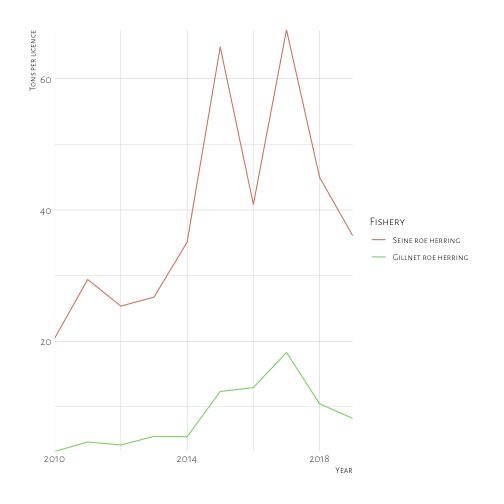
\includegraphics{index_files/figure-latex/quota-per-licence-sog-1.pdf}
\caption{\label{fig:quota-per-licence-sog}Roe herring quota per licence in
the Strait of Georgia by licence type. Source: Compiled season summary
data from DFO reports.}
\end{figure}

\begin{figure}
\centering
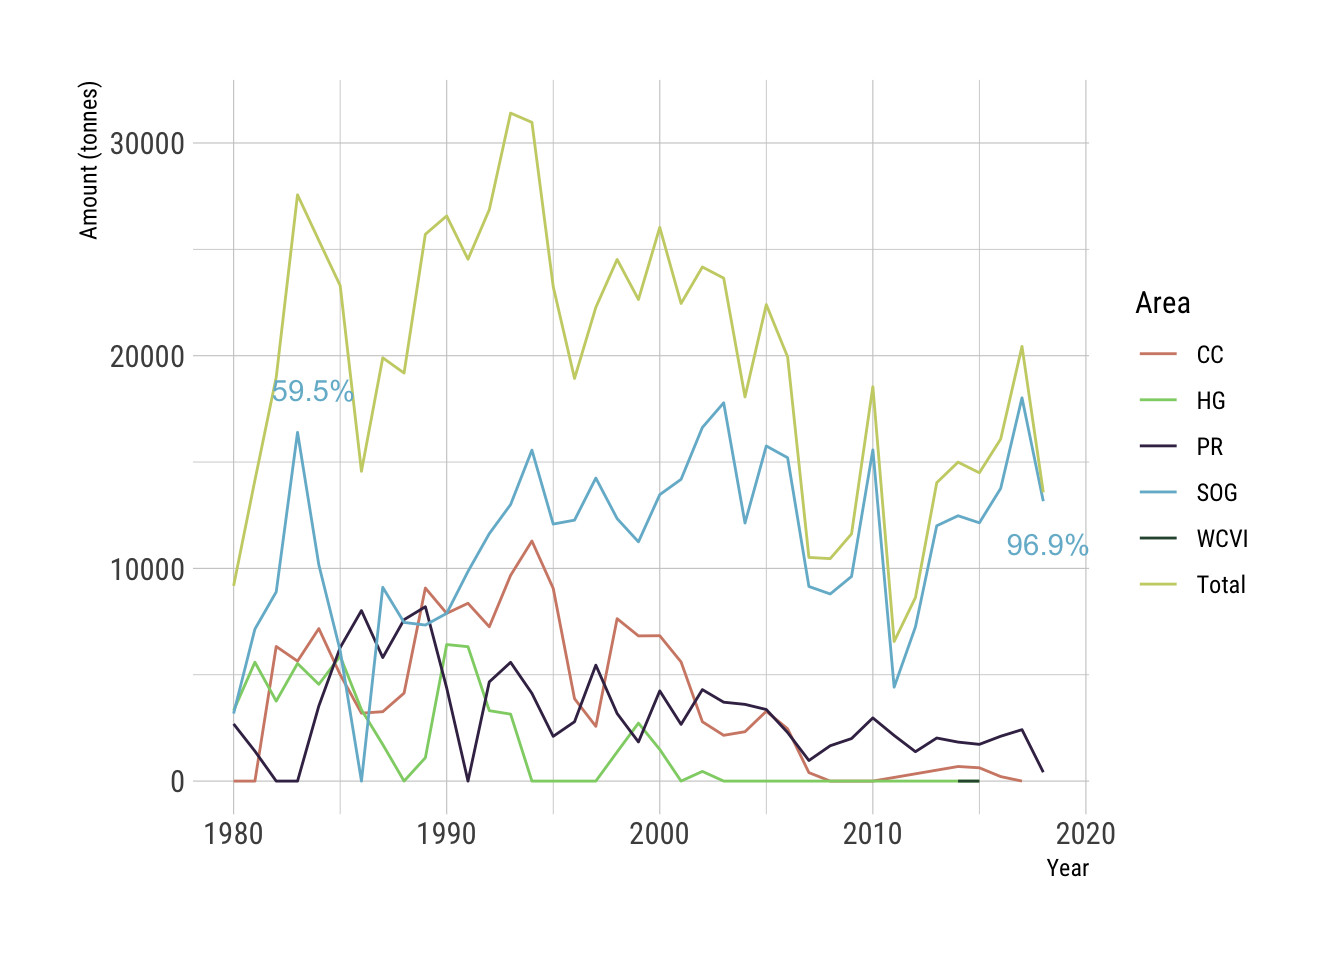
\includegraphics{index_files/figure-latex/catches-area-1.pdf}
\caption{\label{fig:catches-area}Roe herring catches by major fishing area.
Source: Compiled season summary data from DFO reports.}
\end{figure}

Over the past 10 years, the roe herring fishery has fluctuated between
an ex-vessel value of 4 and 17 million (Figure \ref{fig:landed-value}).
Formerly the values were much higher exceeding 100 million CAD in 1987.
In addition, the wholesale value is substantially higher than the landed
value as herring roe is a value-added product.

\begin{figure}
\centering
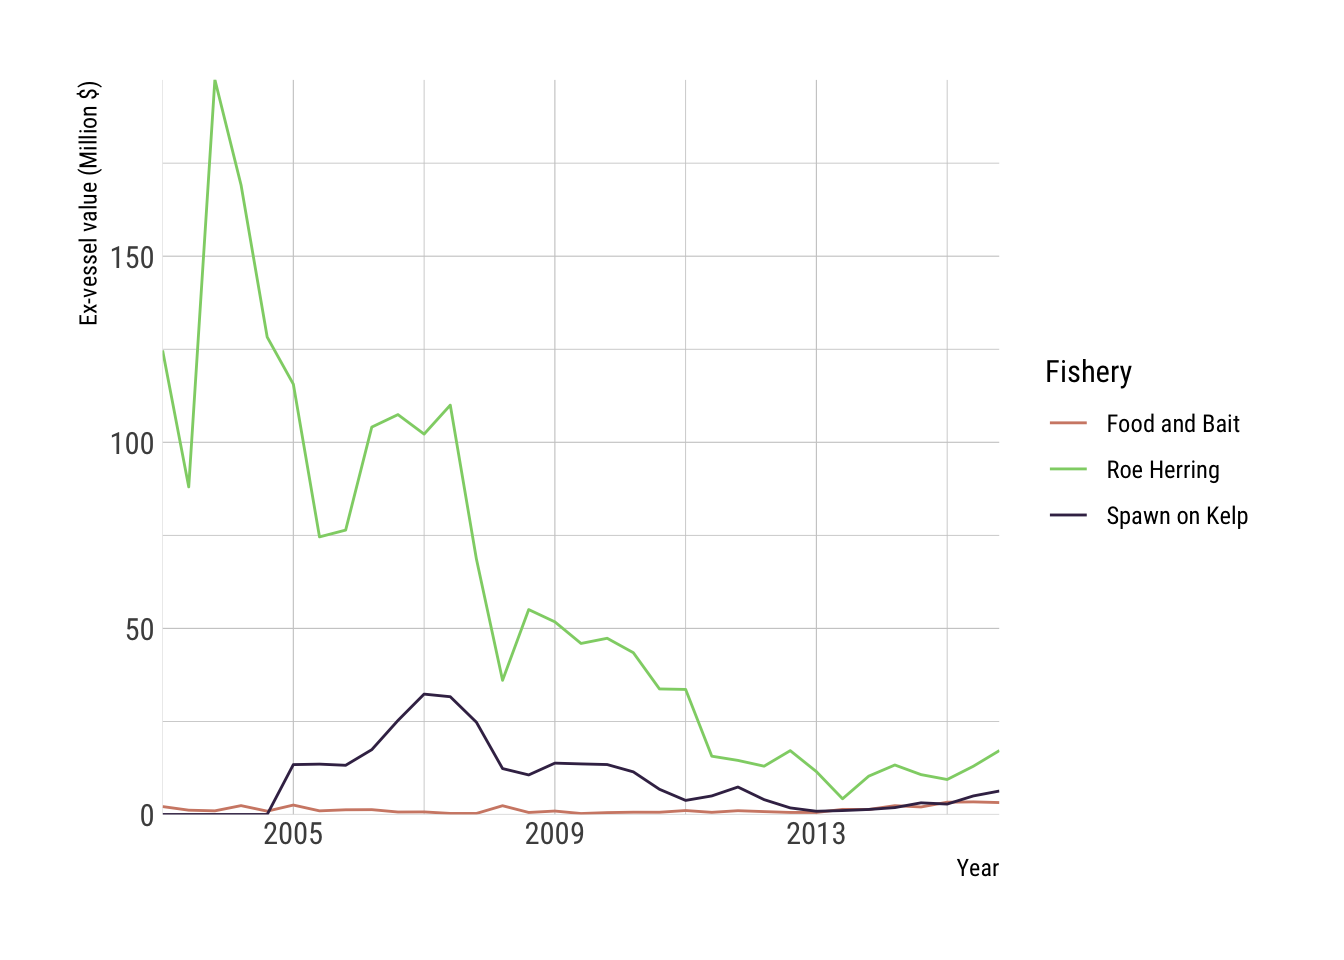
\includegraphics{index_files/figure-latex/landed-value-1.pdf}
\caption{\label{fig:landed-value}Ex-vessel value of herring fisheries.
Source: BC Ministry of Agriculture, 2018.}
\end{figure}

As herring roe is a processed product, it naturally has a higher price
than the raw material of whole herring. In addition, the wholesale value
includes the value of the fishery derived from the processing of roe and
production of fishmeal and fish oil from the herring by-products.

\begin{figure}
\centering
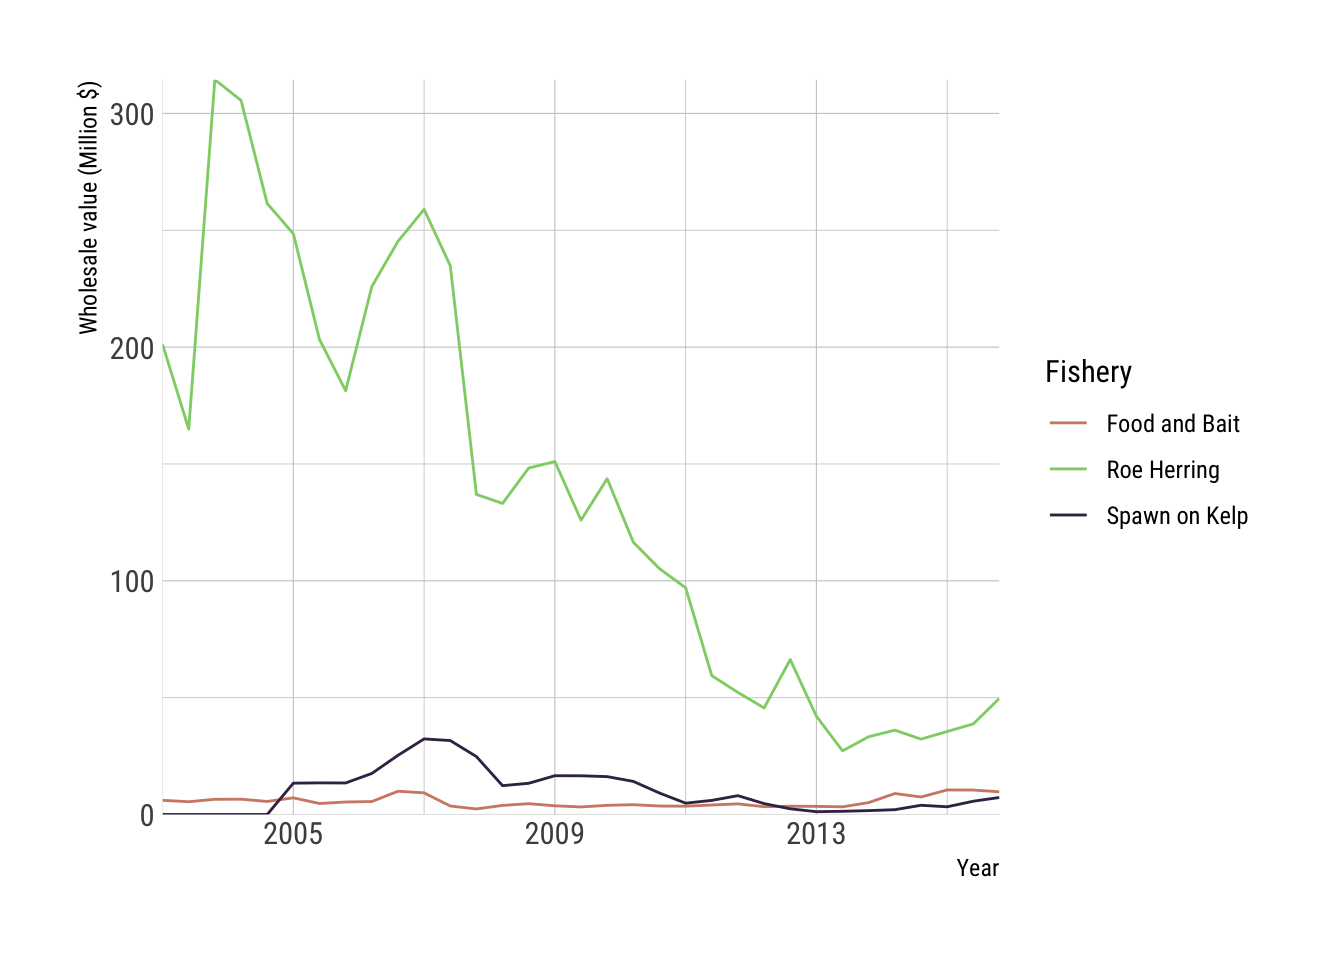
\includegraphics{index_files/figure-latex/wholesale-value-1.pdf}
\caption{\label{fig:wholesale-value}Wholesale value of herring fisheries.
Source: BC Ministry of Agriculture, 2018.}
\end{figure}

The decline in total value of the fishery is both a function of a
decline in landings, and a decline in ex-vessel prices received by
fishers. There is some indication, however, that the prices reported by
fishers does not necessarily indicate lower profitability as processors
have been more willing to pay fishers' fees (e.g., licence costs and
Dockside Monitoring Program costs) thus lowering their cost of fishing
(GSGislason \& Associates Ltd. 2015). Thus, the ex-vessel price
decreases may be partially or wholly offset by the increased costs
covered by processors.

\begin{figure}
\centering
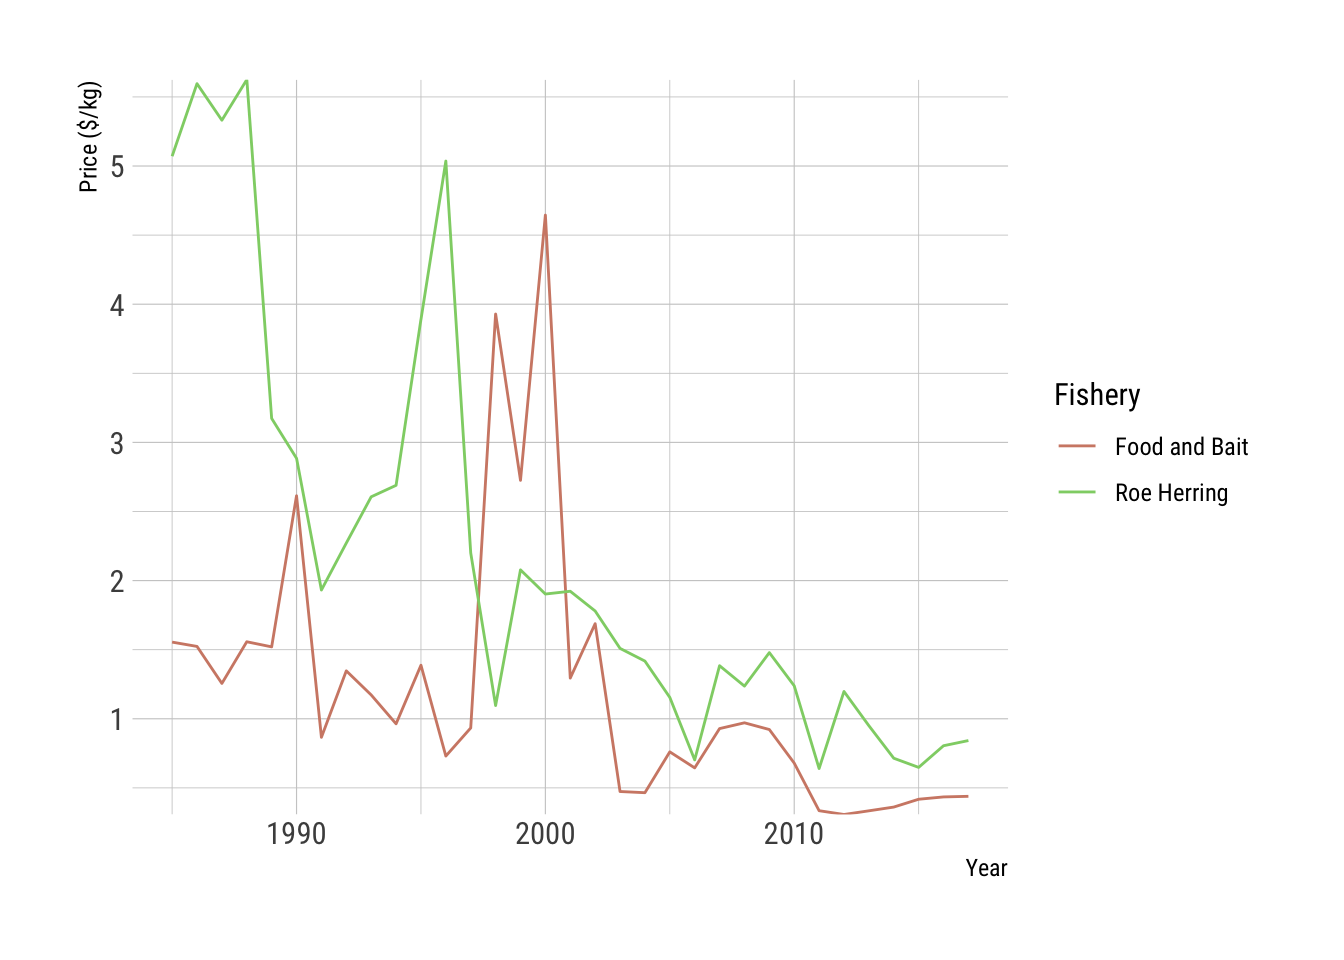
\includegraphics{index_files/figure-latex/ex-vessel-price-1.pdf}
\caption{\label{fig:ex-vessel-price}Ex-vessel price by fishery. Source: BC
Ministry of Agriculture, 2018.}
\end{figure}

There are differences in the price within the roe fishery itself. The
seine fishery generally fetches a lower value than the gillnet fishery
as the gillnet is more selective towards larger and older individuals
which thus have a higher proportion of roe. This was confirmed by an
industry expert, who estimates that 11-13\% of the seine catch by weight
is roe while the gillnet fishery is 14-16\% roe by weight. In some
years, this has led to price differences on the order of 3-4 times
greater for gillnet than seine catches. While there are differences in
the relative price of gillnet caught herring versus seine caught
herring, they both follow the general trend of a large decline in
ex-vessel prices over the past 25 years.

\begin{figure}
\centering
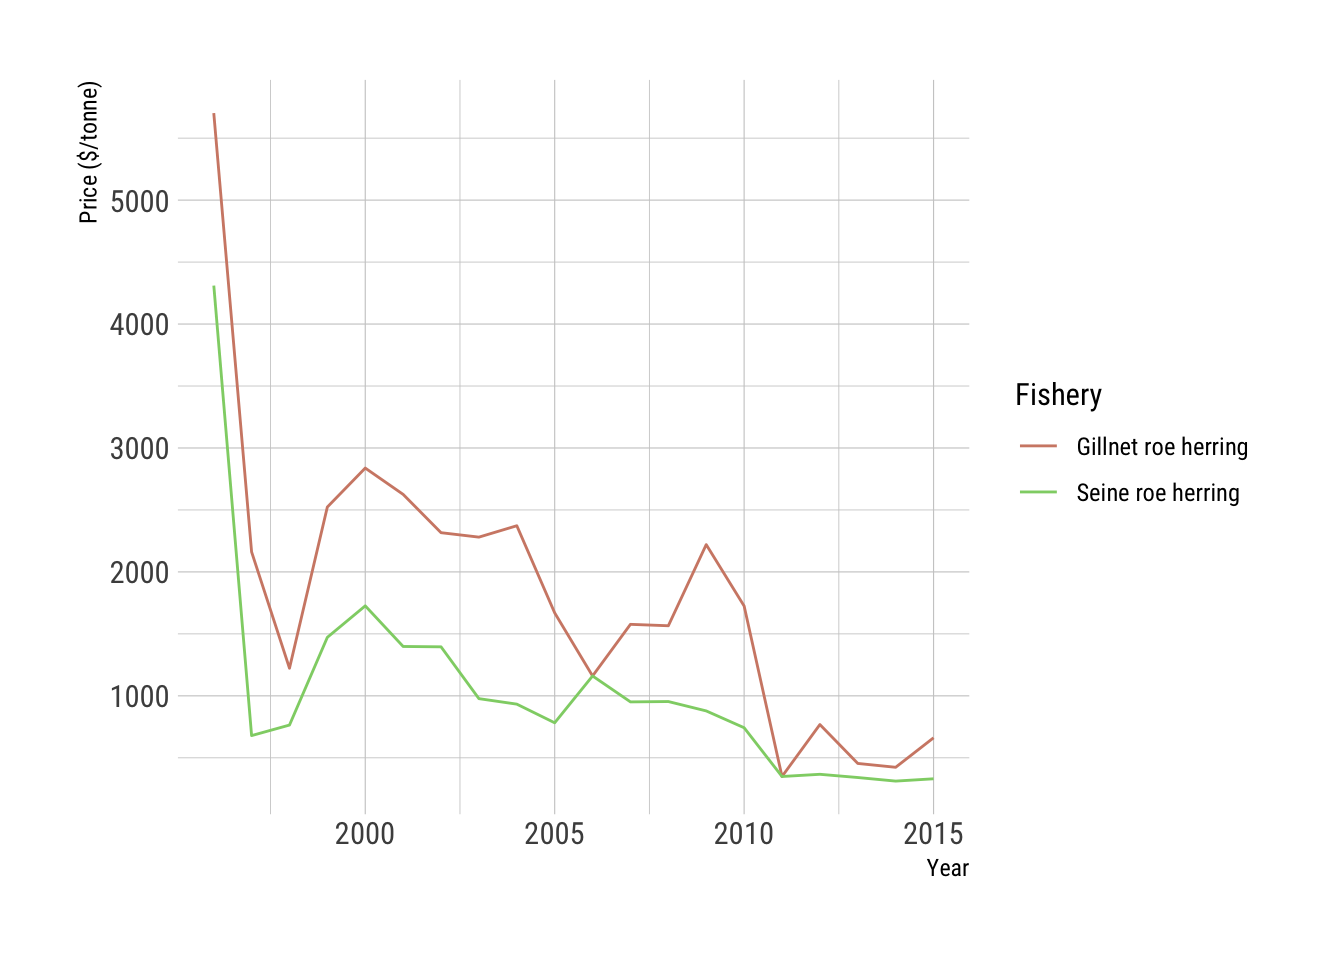
\includegraphics{index_files/figure-latex/ex-vessel-price-gear-1.pdf}
\caption{\label{fig:ex-vessel-price-gear}Coastwide ex-vessel price by gear
for the roe fishery. Source: DFO, 2017}
\end{figure}

\begin{figure}
\centering
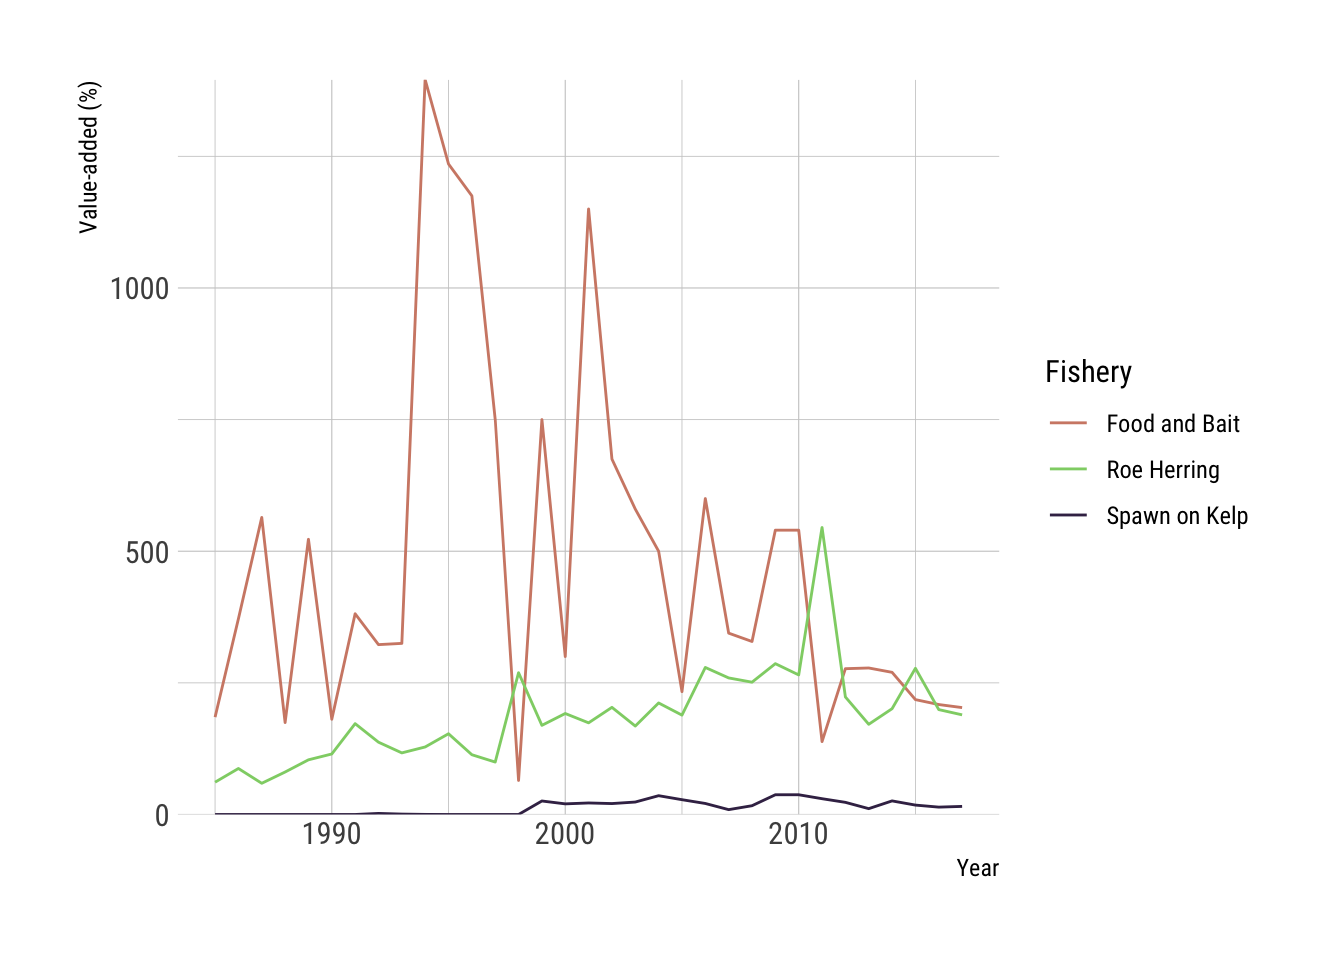
\includegraphics{index_files/figure-latex/value-added-plot-1.pdf}
\caption{\label{fig:value-added-plot}Value-added factor by fishery. Source:
BC Ministry of Agriculture, 2018.}
\end{figure}

\section{Ownership and Licenses}\label{ownership-and-licenses}

The roe herring fishery is managed by a limited entry licence program.
The total allowable catch (TAC) is set at the beginning of the season
based on DFO stock assessments. Before the season the licences must be
pooled into self-selected groups for ease of management where the
gillnet pools must have a minimum of 4 licences per pool, and the seine
fishery must have eight licences per pool but no more than 10 pools
permitted in the Strait of Georgia (DFO 2018b). The TAC is then divided
based on the number of licences in each pool. A seine roe licence can
elect to fish instead in the Food and Bait fishery and then the amount
of catch they would have caught in the roe fishery is switched to allow
them to fish in the Food and Bait fishery.

While the number of roe herring seine licenses is relatively constant,
this does not have a strong relationship to the number of vessels
actually fishing. Most vessels that fish have two licenses stacked on
their vessel. In 2007, only 38 seine vessels registered landings, while
the total fleet of 133 vessels owned 248 licenses (Nelson 2009a). The
number of active fishing vessels in the seine fishery increased to 43
active vessels in 2009 (Lagaron Comba et al. 1999).

\begin{figure}
\centering
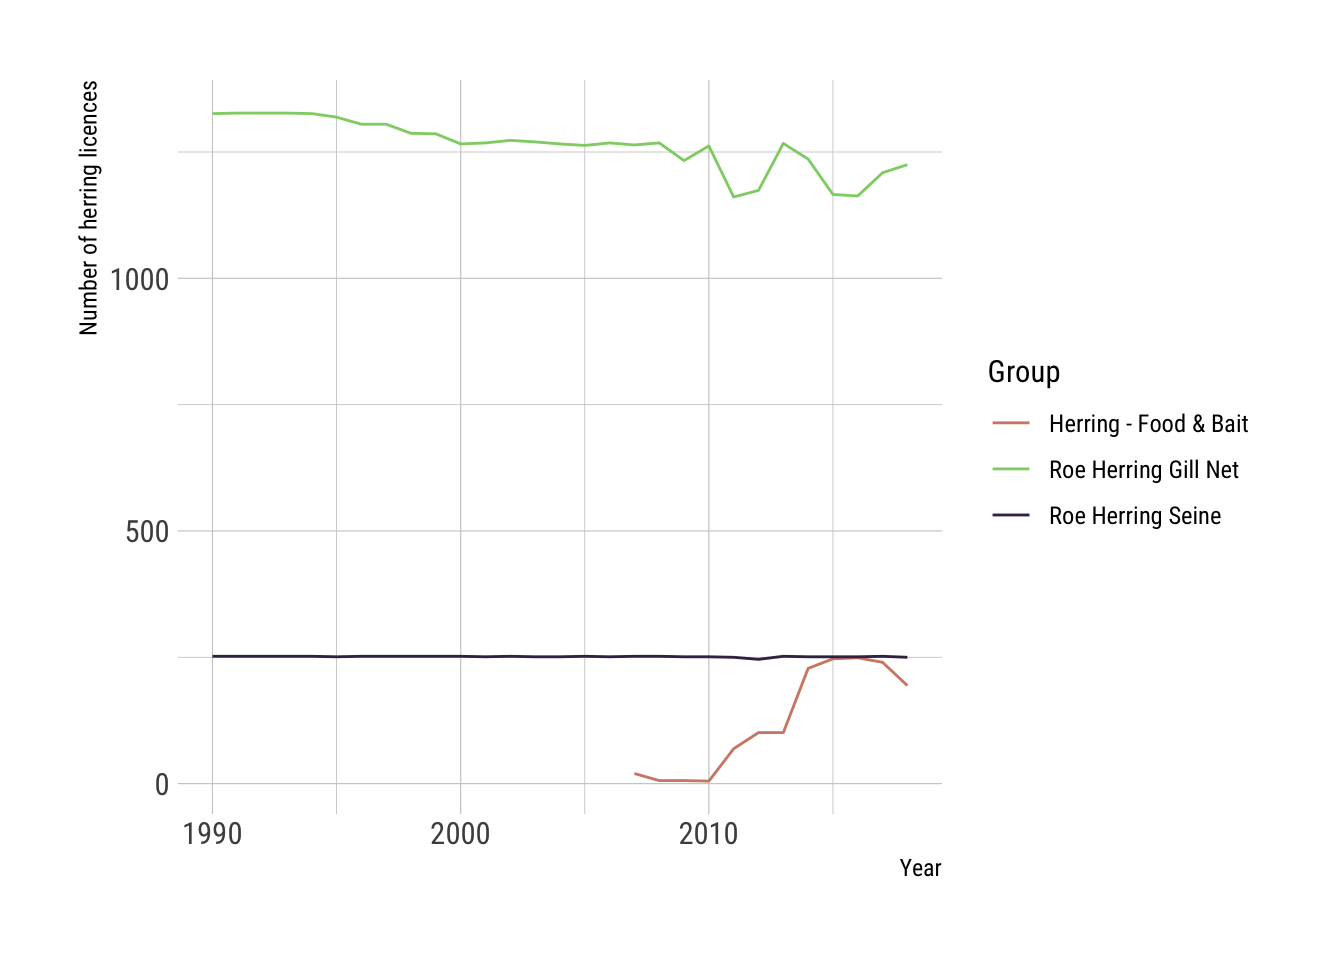
\includegraphics{index_files/figure-latex/licence-number-1.pdf}
\caption{\label{fig:licence-number}Total herring licenses by fishery type}
\end{figure}

The trend in licences by area should be interpreted with caution as the
field is blank for many of the entries in the commercial licence
database. However, there does appear to be movement of licences to the
remaining fishing areas as would be expected as some of the main fishing
areas have been closed for several years (Figure
\ref{fig:licence-area}). This trend is apparent for the Strait of
Georgia as well since 2000 (Figure \ref{fig:licence-sog}).

\begin{figure}
\centering
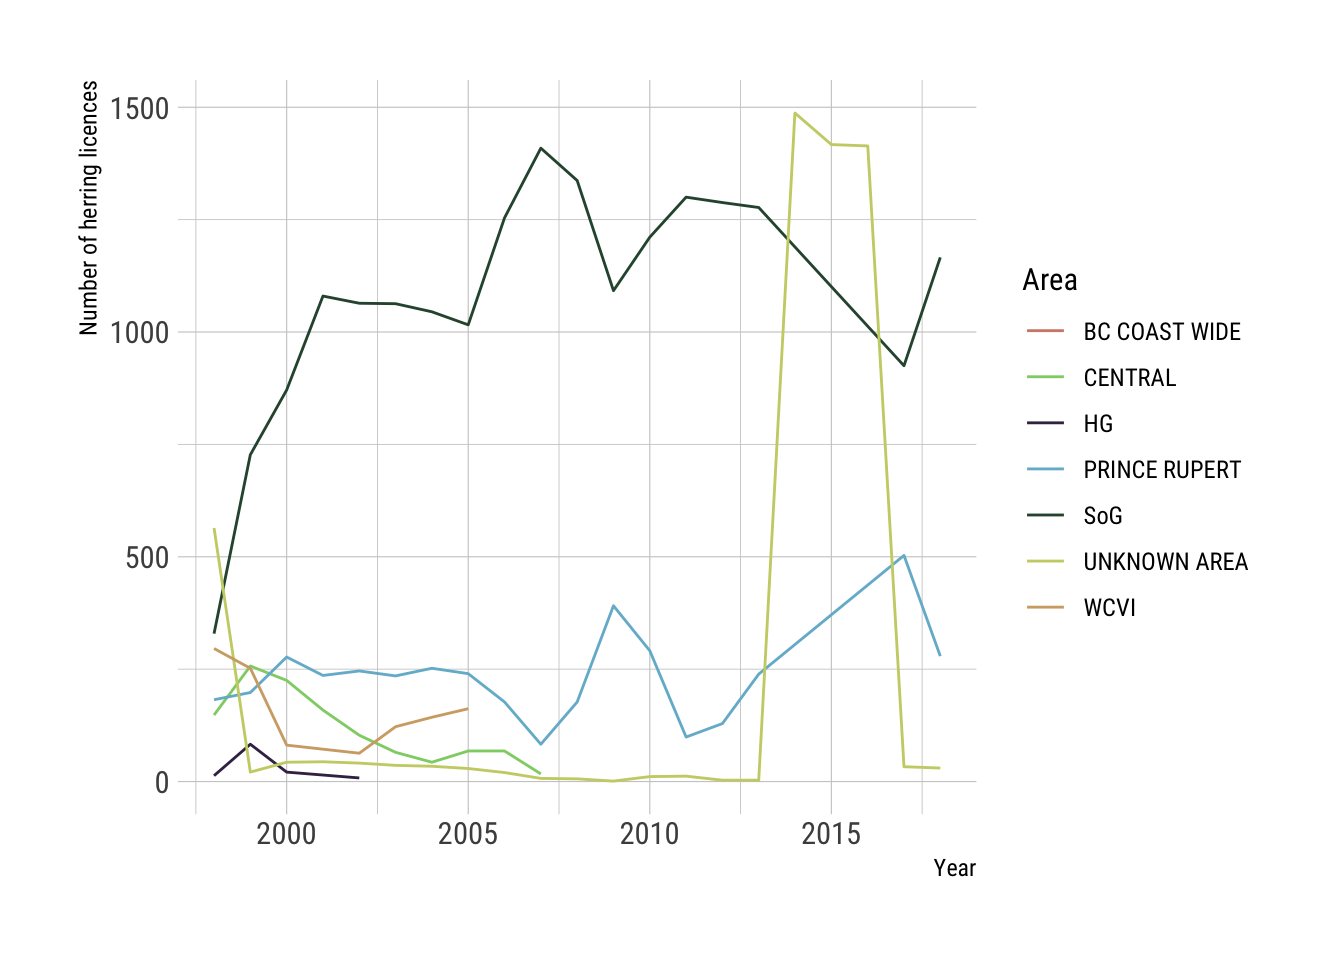
\includegraphics{index_files/figure-latex/licence-area-1.pdf}
\caption{\label{fig:licence-area}Net licence movement for the two main roe
fishing areas.}
\end{figure}

\begin{figure}
\centering
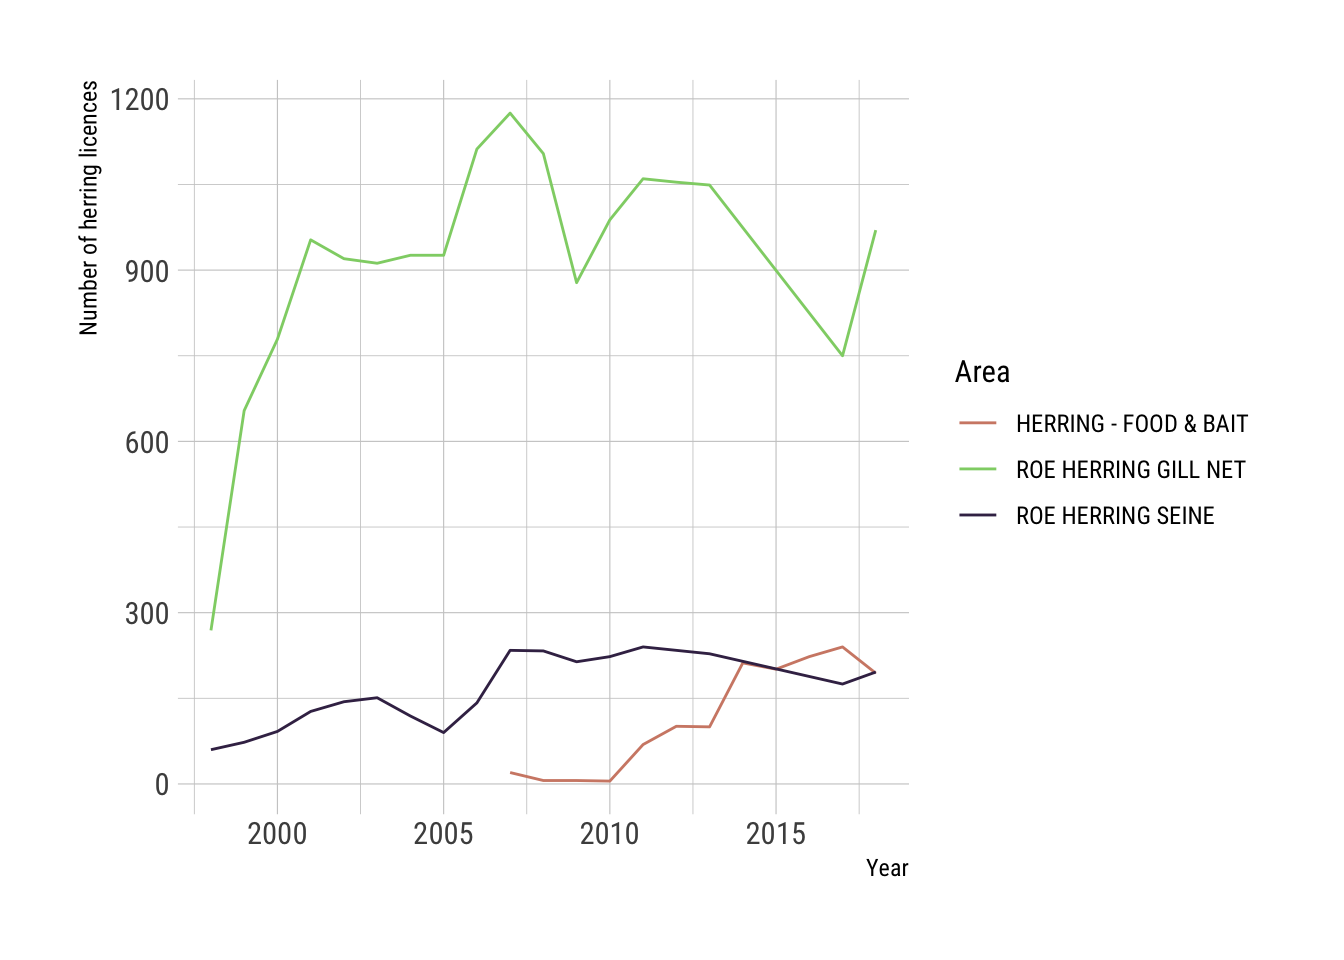
\includegraphics{index_files/figure-latex/licence-sog-1.pdf}
\caption{\label{fig:licence-sog}Number of herring licences in the Strait of
Georgia (excluding special use)}
\end{figure}

\begin{table}

\caption{\label{tab:licence-table}Top 10 companies by herring roe licence ownership (seine and gillnet combined)}
\centering
\begin{tabular}[t]{l|r}
\hline
Company & 2018 Herring roe licences\\
\hline
Jim Pattison Group & 228\\
\hline
Aero Trading Co. Ltd. & 34\\
\hline
Arctic Pearl Ice And Cold Storage Ltd. & 28\\
\hline
Robert Recalma & 28\\
\hline
A-Tlegay Fisheries Society & 25\\
\hline
James Walkus & 25\\
\hline
Salish Seas Fisheries Association & 24\\
\hline
Randy Reifel & 23\\
\hline
Gwabalis Fisheries Society & 18\\
\hline
Corrine Rockl & 16\\
\hline
Other & 1026\\
\hline
\end{tabular}
\end{table}

The largest owner(s) of herring roe licences are the companies belonging
to the Jim Pattison Group (Table \ref{tab:licence-table}). This
concentration in this firm has grown over time and now represents 15\%
of total roe licences. Of these, the Pattison group is more heavily
invested in the seine licences which are worth more and account for more
landings in the roe fisheries (Figure \ref{fig:licence-pattison}).
Therefore, the Pattison Group's expected quota for 2019 in the Strait of
Georgia is 3,823 out of the total 19,498 metric tonnes (19.6\%). Outside
of those owned by the Jim Pattison Group, there is significant
concentration in the top 10 largest herring licence holders.

\begin{figure}
\centering
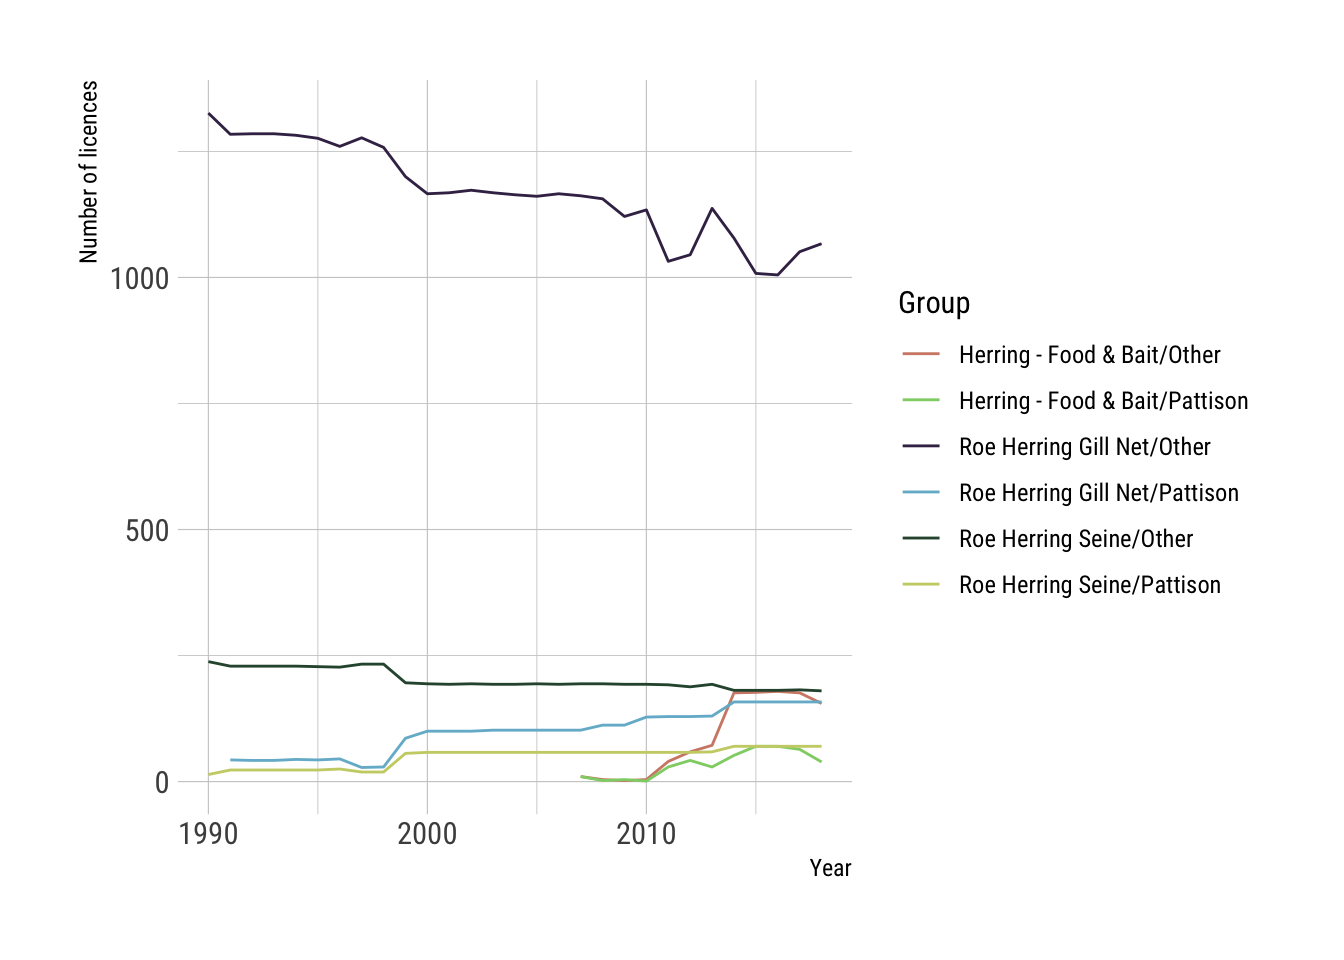
\includegraphics{index_files/figure-latex/licence-pattison-1.pdf}
\caption{\label{fig:licence-pattison}Herring licences owned by the Jim
Pattison Group}
\end{figure}

A standard measure of inequality is the Gini index. The Gini index is a
value between 0 and 1, where 1 represents perfect inequality and 0
represents perfect equality. This measure has been applied to fishing
licences and fleets to measure equity. It was applied to the BC salmon
and herring fisheries and found a large share of corporate control
(Haas, Edwards, and Sumaila 2016). As corporate control has become a
concern for BC, here we investigate the change in inequality in the
fishery over time. There has been a significant increase in the
inequality of the herring licence division over time occurring in both
the seine and gillnet roe fisheries (Figure \ref{fig:gini-time}).

\begin{figure}
\centering
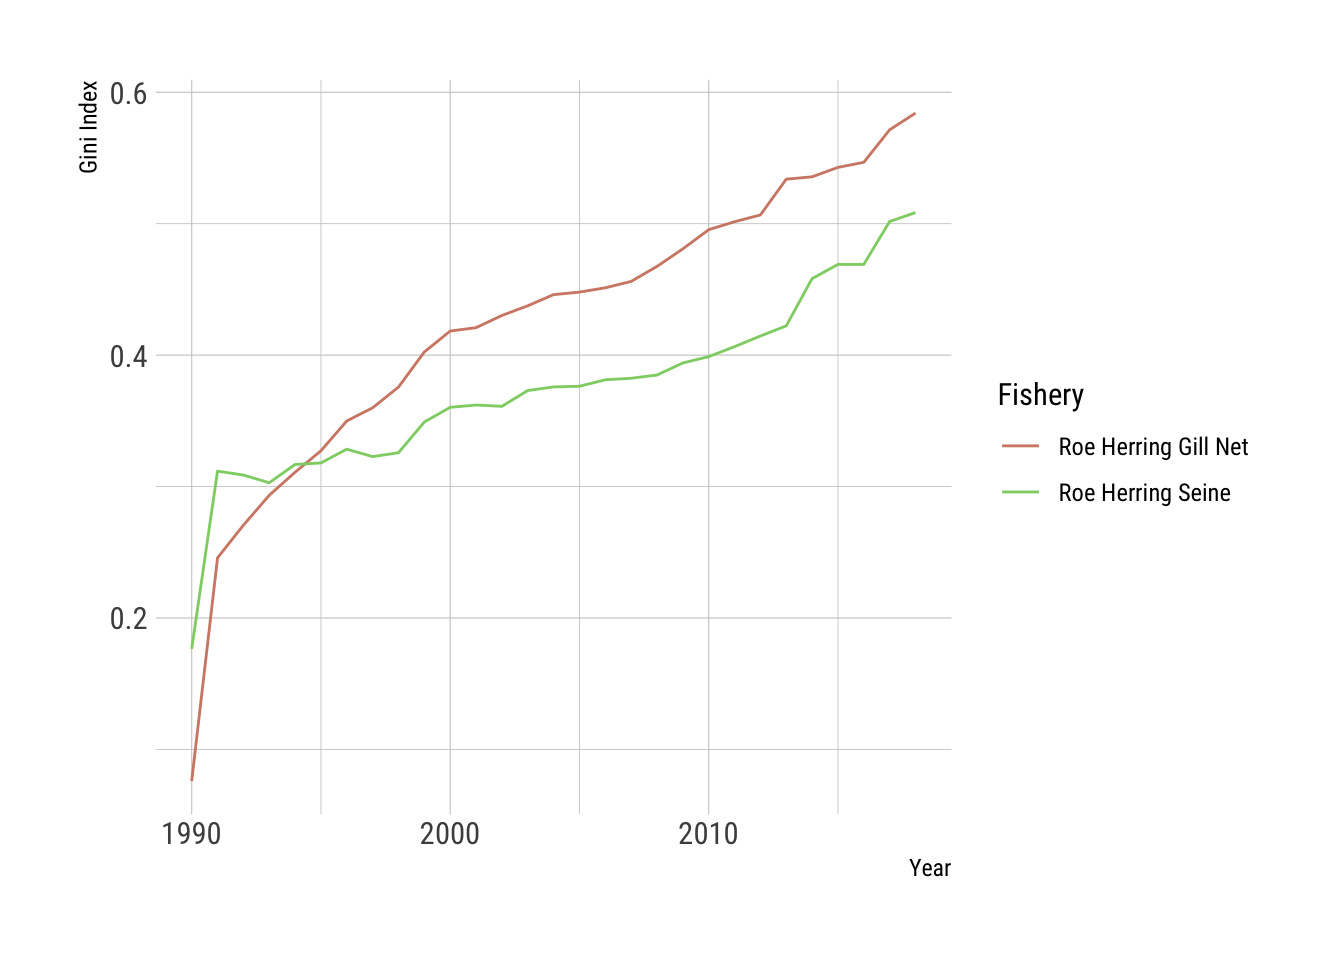
\includegraphics{index_files/figure-latex/gini-time-1.pdf}
\caption{\label{fig:gini-time}Gini coefficient for roe herring licences}
\end{figure}

The value of roe herring licences for both the gillnet and seine have
declined substantially since high levels in the late 1990s and early
2000s. The outright licence fees are so much lower that the lease value
of these licences has dropped to near zero. By industry accounts, there
is very little leasing of licences in the gillnet fishery and almost
none in the seine fishery.

\begin{figure}
\centering
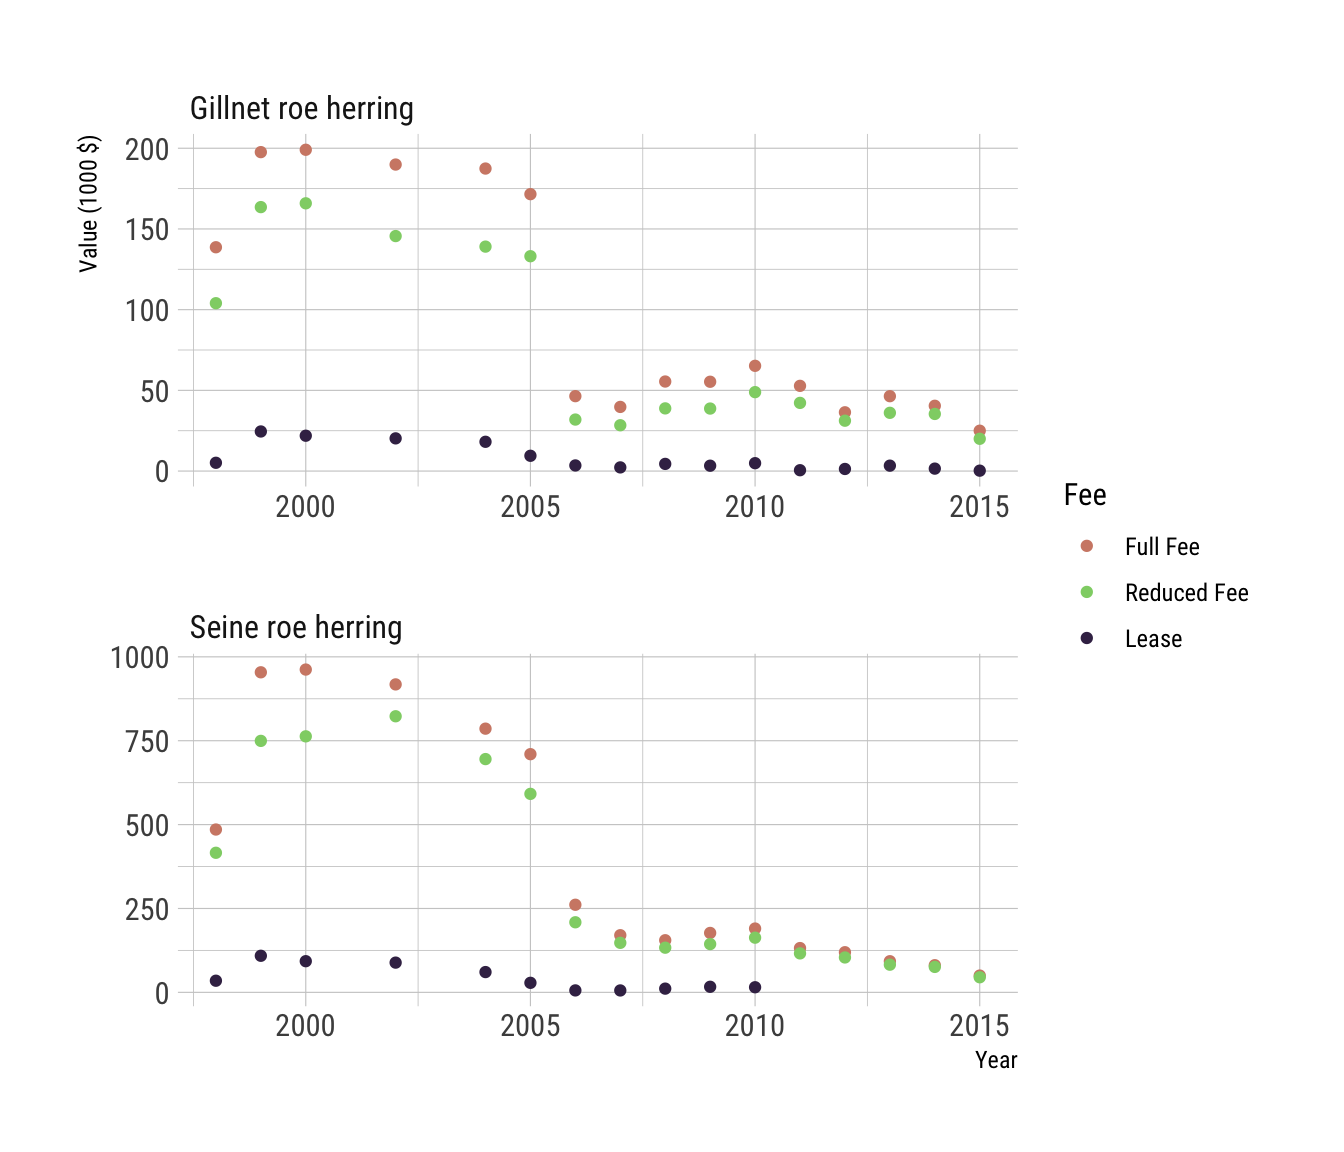
\includegraphics{index_files/figure-latex/licence-value-1.pdf}
\caption{\label{fig:licence-value}Herring licence values by fishery type and
fee. Source: Compiled from various reports of Nelson Bros Fisheries
Ltd.}
\end{figure}

\section{How does the roe herring fishery stack
up?}\label{how-does-the-roe-herring-fishery-stack-up}

Based on data from BC statistics (AgriService BC 2018), wild salmon
processing generates \textasciitilde{}4x as much in wages as herring
processing does. In 2016 when wild salmon and herring catches were
comparable (24,700 tonnes and 24,100 tonnes, respectively), wild salmon
generated 5.4x as many processing jobs (annual average of 1,400 compared
to 332 for herring) (AgriService BC 2018). Similarly, these jobs
resulted in higher wages for wild salmon that generated just over
\$2,000/tonne processed while herring was \$525/tonne.

\begin{figure}
\centering
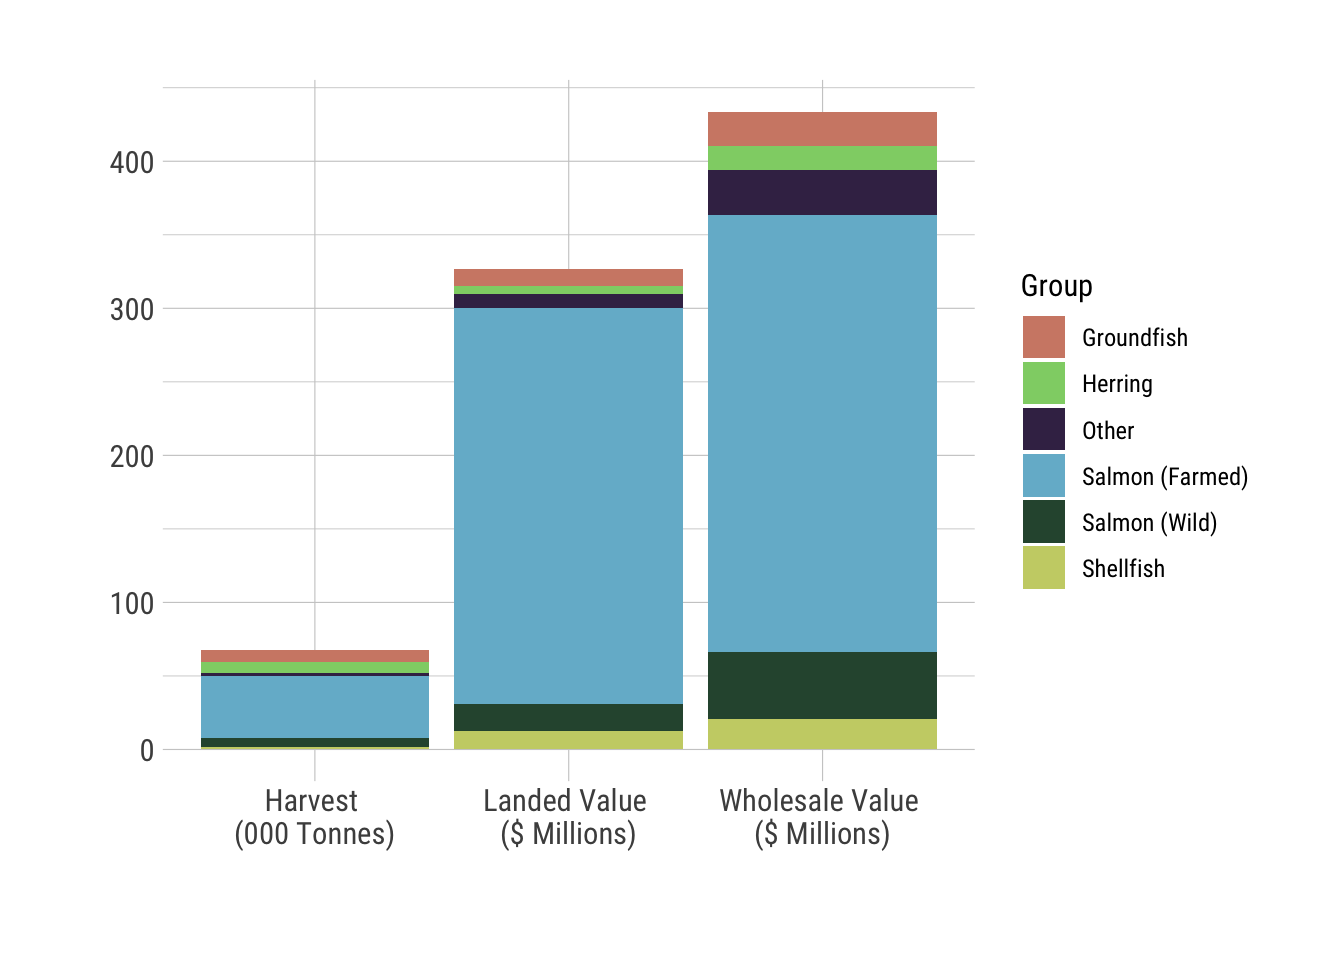
\includegraphics{index_files/figure-latex/bc-seafood-1.pdf}
\caption{\label{fig:bc-seafood}Harvest and value (landed and wholesale) of
BC seafood production averaged over 2014-2016. Source: BC AgriService
2017.}
\end{figure}

Compared to other valuable species in the Strait of Georgia, such as
salmon, herring catches are higher in tonnage but lower in value.

\begin{figure}
\centering
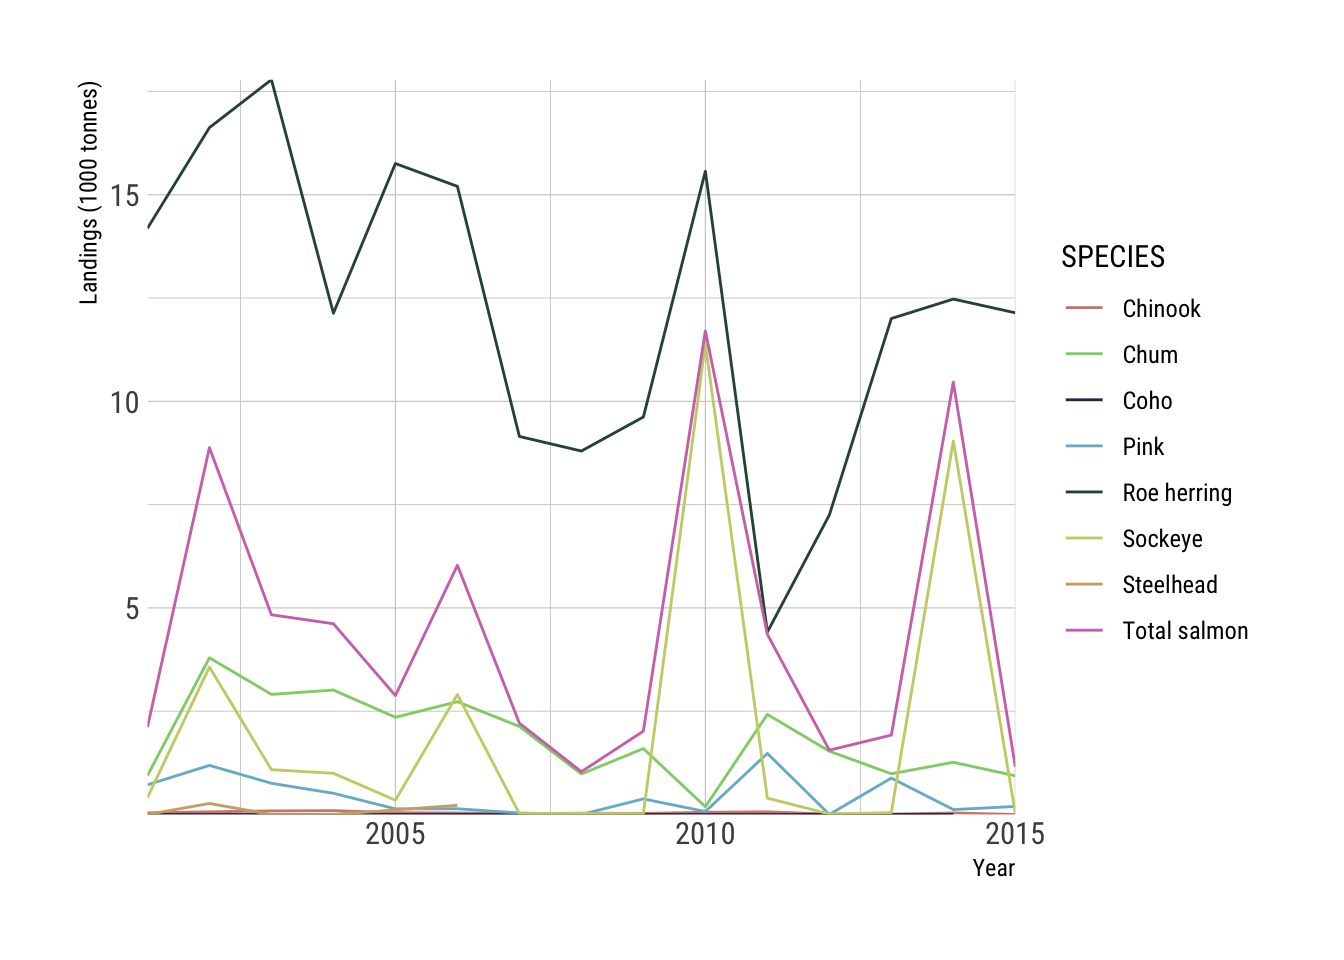
\includegraphics{index_files/figure-latex/salmon-district-amount-1.pdf}
\caption{\label{fig:salmon-district-amount}Commercial salmon landings in the
Strait of Georgia. Source: DFO, 2017.}
\end{figure}

\begin{figure}
\centering
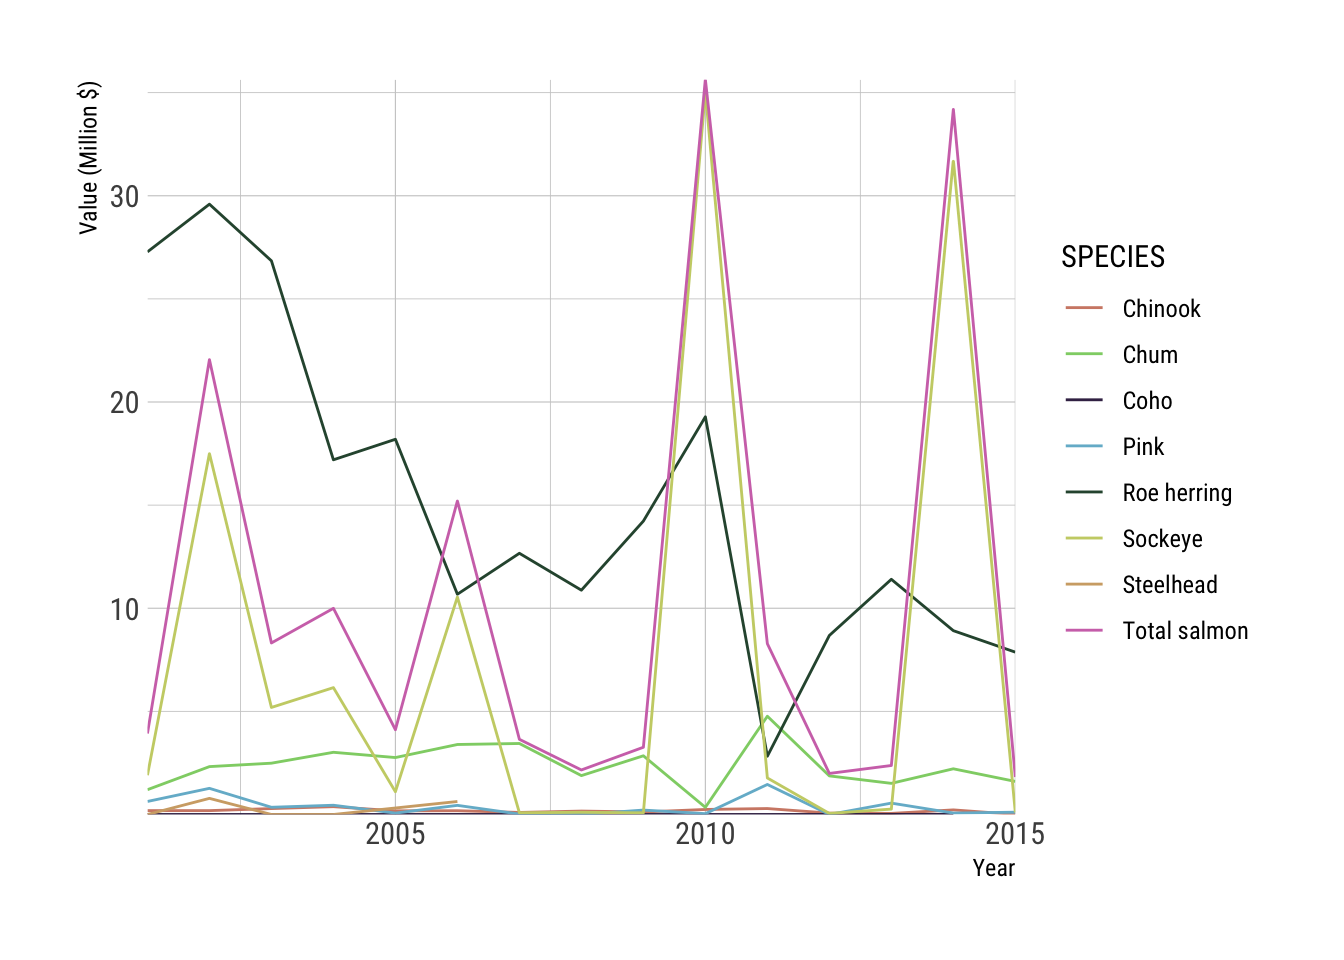
\includegraphics{index_files/figure-latex/salmon-district-value-1.pdf}
\caption{\label{fig:salmon-district-value}Commercial salmon ex-vessel value
in the Strait of Georgia. Source: DFO, 2017.}
\end{figure}

In addition to the commercial fishery in the Strait of Georgia, there is
a valuable recreational fishery for salmon in the Strait of Georgia.
While other areas of the BC coast account for larger numbers of salmon
caught by recreational fishers, the Strait of Georgia has the most
fishing effort recorded in boat days for those areas with data (Note:
Northern and Central coast data was not available for this year). One
crude measure of the value of the recreational fisheries is the value
they produce in fish themselves if the fish was sold commercially
(Colquhoun and Ridge Partners 2015). This measure of value is crude and
non-inclusive as recreational fishing is not solely for the production
of fish, and countless studies have shown that the value recreational
fishing gives to society far exceeds this `product' value. Nevertheless,
the product value of recreational tidal water salmon fisheries in BC is
over 15 million dollars annually, with the Strait of Georgia accounting
for 1.3 million dollars of this.

\begin{figure}
\centering
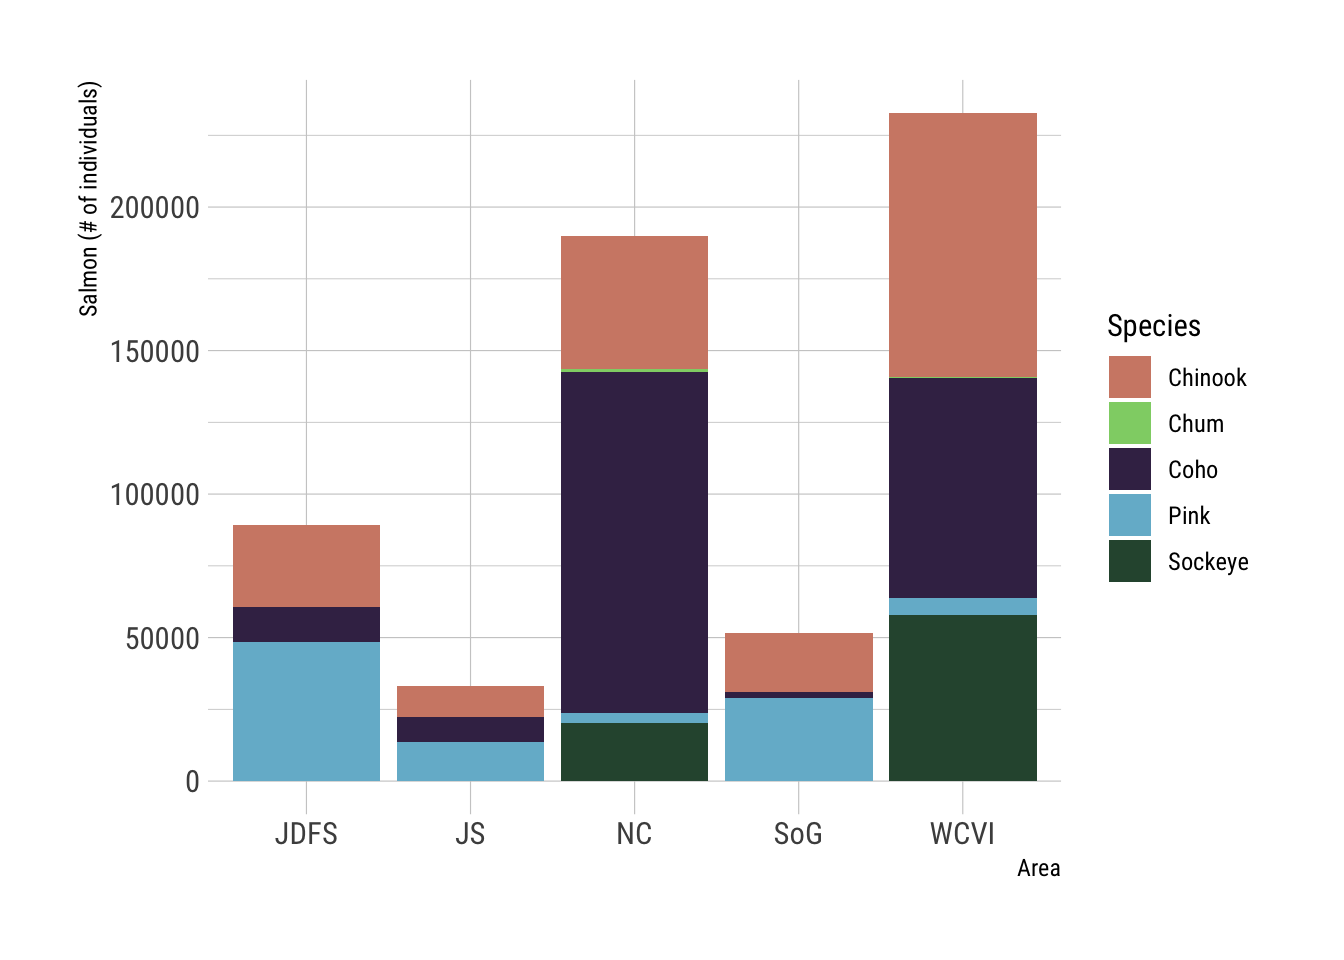
\includegraphics{index_files/figure-latex/recreational-fishes-1.pdf}
\caption{\label{fig:recreational-fishes}Recreational salmon landings (tidal
water) in BC by area for 2009. JDFS: Juan de Fuca Strait; JS: Johnstone
Strait; NC: North Central Coast; SoG: Strait of Georgia; WCVI: West
Coast of Vancouver Island. Source: DFO, 2016}
\end{figure}

\begin{figure}
\centering
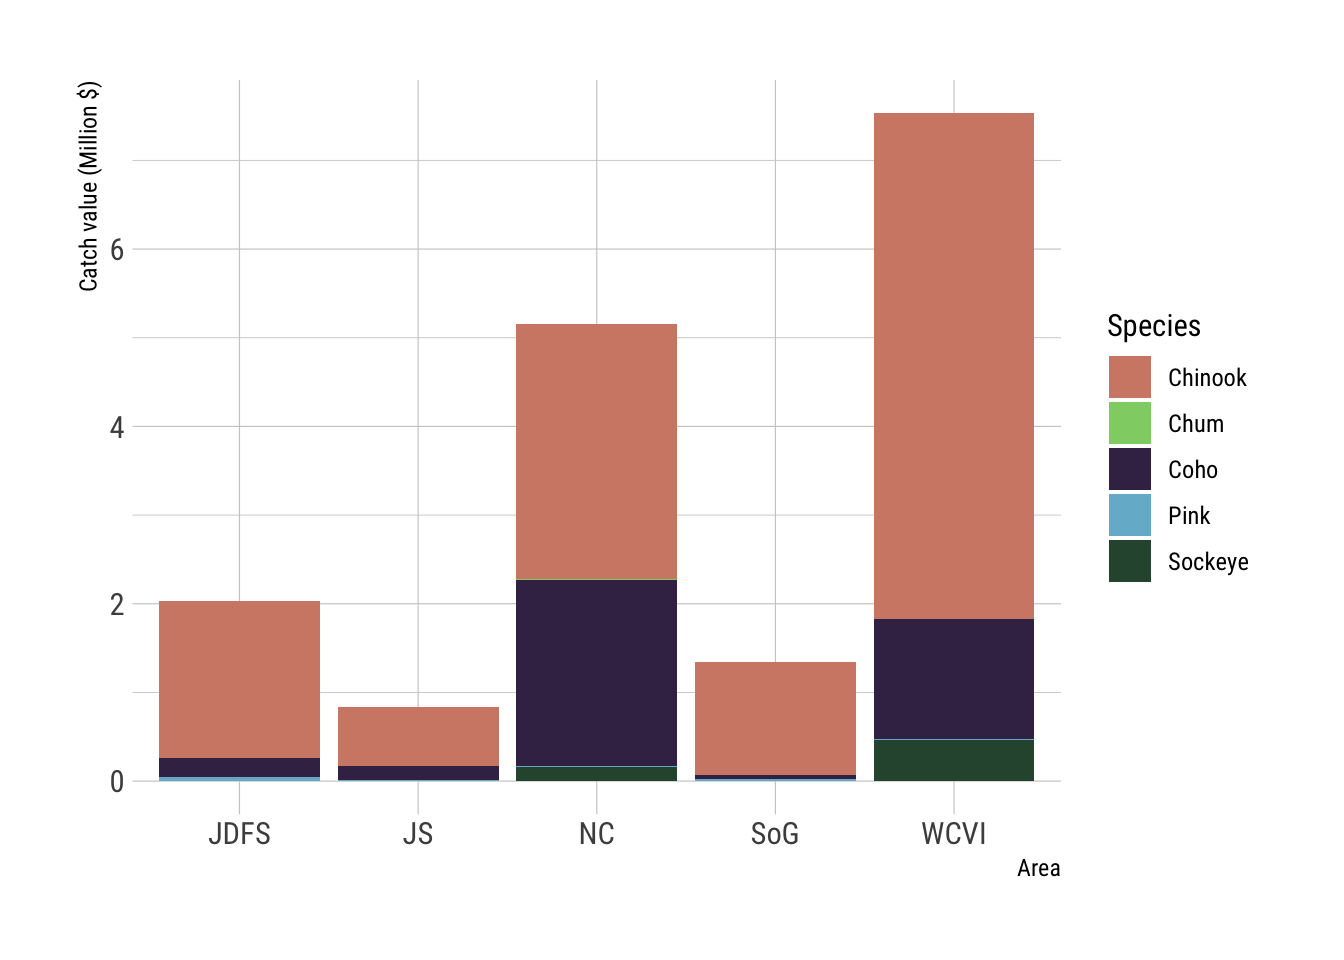
\includegraphics{index_files/figure-latex/recreational-value-1.pdf}
\caption{\label{fig:recreational-value}Recreational salmon value (tidal
water) in BC by area for 2009. JDFS: Juan de Fuca Strait; JS: Johnstone
Strait; NC: North Central Coast; SoG: Strait of Georgia; WCVI: West
Coast of Vancouver Island. Source: Estimated based on commercial value
of salmon and landings data from DFO, 2016}
\end{figure}

\textbackslash{}begin\{figure\}
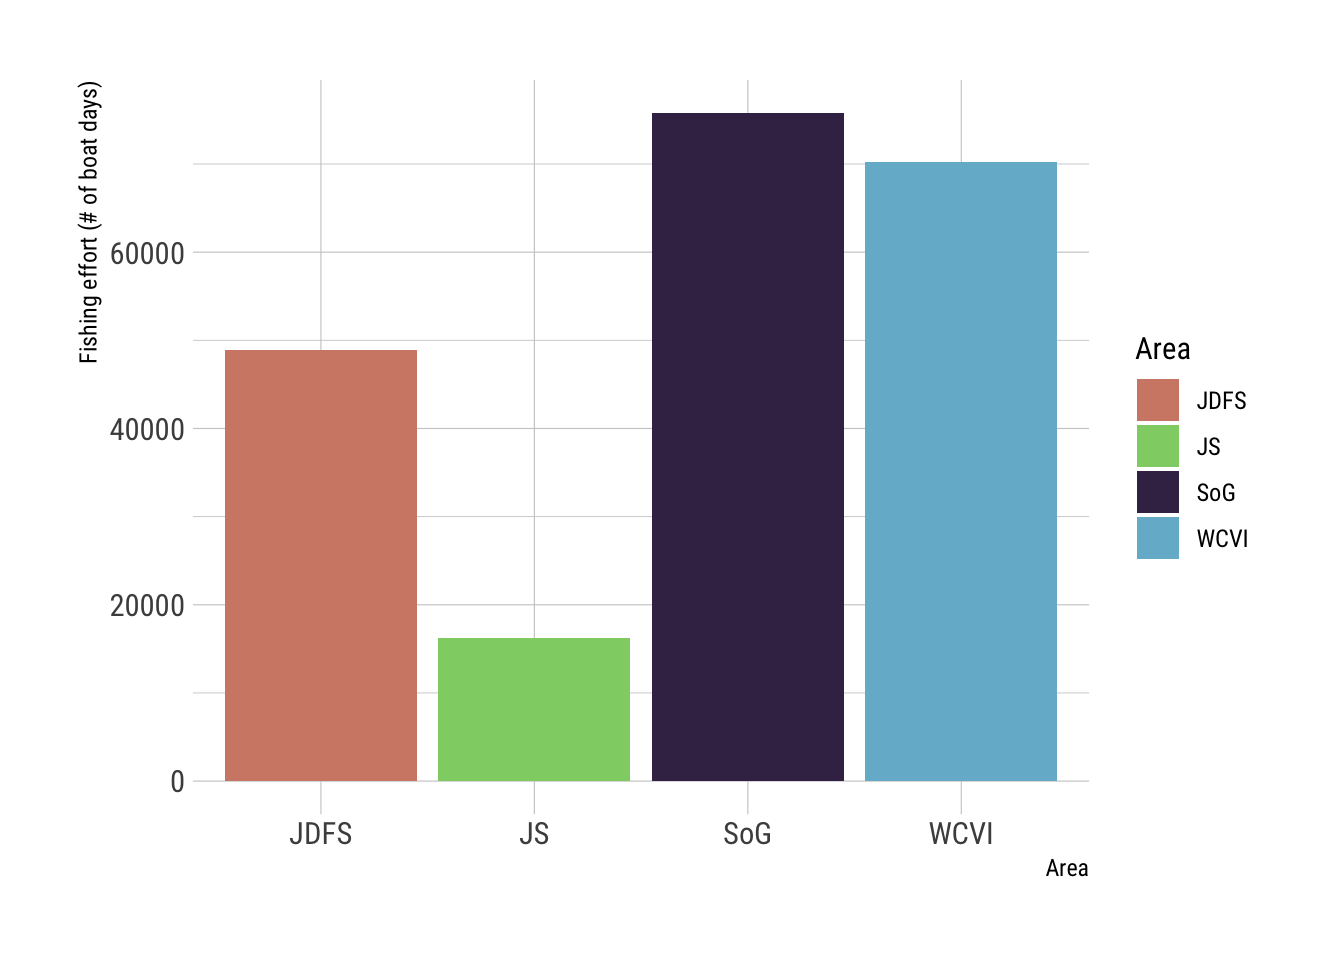
\includegraphics{index_files/figure-latex/recreational-effort-1}

\section{Going forward: A look into closing the roe herring
fishery}\label{going-forward-a-look-into-closing-the-roe-herring-fishery}

Pacific Wild asked the author to consider a temporary closure of the
fishery with the aim of protecting the ecosystem as herring plays an
important role in many of its predators' diets. This closure has been
proposed to rebuild herring stocks and protect the species that rely
upon herring in this ecosystem. The following details options based on
previous experience of temporary fishery closures and licence buy-backs
in Canada.

The first example will draw directly from the BC herring fishery. In
recent years, the roe herring fishery has had quota assigned to fishing
areas where a fishery opening did not occur (Government of Canada 2014).
Many fishers had purchases licences for these areas prior to the fishery
opening and were not allowed to fish them. In these cases, the fishers
were reimbursed for the cost of the licence (Government of Canada 2014),
but not for any extra costs or the lost income of the fishery. In this
case, the cost of reimbursement for the licences for the 2019 season is
expected to be a maximum of 1,256,360 (assuming that all licences are
full fee, which gives a maximum value rather than the true value).

For a temporary closure, the government could act in ways that is has in
the past when extenuating circumstances warrant a closure of a fishery.
In this case, the compensation that fishers receive is closely in line
with what fishers receive for employment insurance payments (Emery 1992;
CBC News 2007). These payments take into account the regional rate of
unemployment, earnings from fishing, earnings from other activities, and
a predetermined allowed maximum weekly amount (Government of Canada
2019). The maximum weekly amount in 2019 is \$1,021 a week (Government
of Canada 2019). If a fisher's total weekly earnings was less than this,
they would use that amount in its place. The amount paid is 55\% of the
lower of the two numbers, thus making the maximum amount paid per fisher
\$562. As we determined the full-time equivalent contribution of the roe
herring fishers in the Strait of Georgia and the processing jobs they
generate, we can use these FTEs and the maximum weekly amount paid to
compensate for the loss of this fishery to fishers and processors as has
been done with other fishery closures (Emery 1992). Therefore, the cost
of income supplements for a temporary closure of the fishery is
estimated to be \$175,344.

Licenses are retired in fisheries to reduce capacity to a more
ecologically or economically sustainable level, or to permanently close
the fishery. The roe herring fishery is a limited entry licence fishery
similar to the Pacific salmon fisheries in BC. Therefore, we can use the
salmon fishery licence buybacks as an option for this fishery if there
are believed to be benefits from reducing capacity. From 1996 to 2000,
1,406 salmon licences (34\% of licenses in 1996) were retired at a total
cost of \$195 million dollars (\textasciitilde{}\$138,000 per licence).
As the roe herring licences are at a near all-time low cost, it would
likely be less expensive to remove these licenses and there are less
licenses to begin with in the fishery (total roe herring licenses of
1,475). In addition, the average seine herring license is valued at
approximately \$50,000 and the average gillnet herring licence is valued
at \$25,000. Therefore, the cost of retiring these licenses would likely
be less than it was for salmon. The effectiveness of a licene retirement
program is predicated on the limiting of expansion of effort in the
remaining fleet. Therefore, a licence retirment program would not be
successful without additional caps on fishing capacity and effort.

These strategies may not fully consider the potential strategic
importance of the fishery. The herring fishery may be of particular
strategic importance as it is a fishing and processing activity that
occurs at an off-peak time of year for the fishing industry, and keeps
income flowing to keep people employed closer to year-round. This may be
especially important for the administrative side of the industry and
provides additional weeks of employment to fishers and processors
(GSGislason \& Associates Ltd. 2015). Without these additional weeks,
the increased precariousness of employment could lead to higher turnover
of staff.

\section{Conclusion}\label{conclusion}

The roe herring fishery's catches declined substantially over the 2000s,
but have begun to increase again since 2011. However, the value the
fishery has not responded in the same way due to decreasing prices paid
to the fishers (ex-vessel value), and the decline in value of the main
product of the fishery: herring roe. The fishery is now concentrated
solely in the Strait of Georgia.

\section*{References}\label{references}
\addcontentsline{toc}{section}{References}

\hypertarget{refs}{}
\hypertarget{ref-AgriServiceBC2017}{}
AgriService BC. 2017. ``British Columbia Seafood Industry - Year in
Review 2016.'' Victoria, BC.
\url{http://www.env.gov.bc.ca/omfd/reports/index.html}.

\hypertarget{ref-AgriServiceBC2018}{}
---------. 2018. ``2016 British Columbia Fish Processing Employment.''
Victoria, BC: Government of BC.
\href{https://www2.gov.bc.ca/gov/content/industry/agriculture-\%20seafood/statistics/industry-and-sector-profiles}{https://www2.gov.bc.ca/gov/content/industry/agriculture- seafood/statistics/industry-and-sector-profiles}.

\hypertarget{ref-BCMinistryofAgriculture2018}{}
BC Ministry of Agriculture. 2018. ``British Columbia herring harvest,
landed value and wholesale value (1985-2017).'' Victoria: BC Ministry of
Agriculture.

\hypertarget{ref-CBCNews2007}{}
CBC News. 2007. ``Feds fund compensation program for ice-stricken
fishermen.''
\url{https://www.cbc.ca/news/canada/newfoundland-labrador/feds-fund-compensation-program-for-ice-stricken-fishermen-1.664160}.

\hypertarget{ref-Colquhoun2015}{}
Colquhoun, Ewan, and Ridge Partners. 2015. ``Measuring the economic
value of recreational fishing at a national level.'' Brisbane,
Australia: Fisheries Research \& Development Corporation.
\url{www.frdc.com.au}.

\hypertarget{ref-DFO2015}{}
DFO. 2010. ``Pacific Region Integrated Fisheries Management Plan Pacific
Herring 2010/2011.'' Fisheries; Oceans Canada.
\url{http://www.pac.dfo-mpo.gc.ca/fm-gp/mplans/2013/herring-hareng-2012-2013-eng.pdf}.

\hypertarget{ref-FisheriesandOceansCanada2011}{}
---------. 2011. ``Pacific Region Integrated Fisheries Management Plan:
Pacific Herring 2011/2012.'' Fisheries; Oceans Canada.
\url{http://www.dfo-mpo.gc.ca/Library/344588.pdf}.

\hypertarget{ref-DFO2015a}{}
---------. 2012. ``Pacific Region Integrated Fisheries Management Plan
Pacific Herring 2012/2013.'' Fisheries; Oceans Canada.
\url{http://www.pac.dfo-mpo.gc.ca/fm-gp/mplans/2013/herring-hareng-2012-2013-eng.pdf}.

\hypertarget{ref-DFO2015b}{}
---------. 2015a. ``Pacific Region Integrated Fisheries Management Plan
Pacific Herring 2013/2014.'' Fisheries; Oceans Canada.
\url{http://www.pac.dfo-mpo.gc.ca/fm-gp/mplans/2013/herring-hareng-2012-2013-eng.pdf}.

\hypertarget{ref-DFO2015c}{}
---------. 2015b. ``Pacific Region Integrated Fisheries Management Plan
Pacific Herring 2014/2015.'' Fisheries; Oceans Canada.
\url{http://www.pac.dfo-mpo.gc.ca/fm-gp/mplans/2013/herring-hareng-2012-2013-eng.pdf}.

\hypertarget{ref-DFO2015d}{}
---------. 2015c. ``Pacific Region Integrated Fisheries Management Plan
Pacific Herring 2015/2016.'' Fisheries; Oceans Canada.
\url{http://www.pac.dfo-mpo.gc.ca/fm-gp/mplans/2013/herring-hareng-2012-2013-eng.pdf}.

\hypertarget{ref-DFO2015e}{}
---------. 2016. ``Pacific Region Integrated Fisheries Management Plan
Pacific Herring 2016/2017.'' Fisheries; Oceans Canada.
\url{http://www.pac.dfo-mpo.gc.ca/fm-gp/mplans/2013/herring-hareng-2012-2013-eng.pdf}.

\hypertarget{ref-Report2009}{}
---------. 2018a. ``Pacific Region Integrated Fisheries Management Plan
Pacific Herring 2017/2018.'' Fisheries; Oceans Canada.
doi:\href{https://doi.org/10.4324/9780203928660}{10.4324/9780203928660}.

\hypertarget{ref-DFO2018}{}
---------. 2018b. ``Pacific Region Integrated Fisheries Management Plan
Pacific Herring 2018/2019.'' Vancouver, BC: Fisheries; Oceans Canada.

\hypertarget{ref-Emery1992a}{}
Emery, Claude. 1992. ``The northern cod crisis (BP-313E).'' Political;
Social Affairs Division.
\url{http://publications.gc.ca/Collection-R/LoPBdP/BP/bp313-e.htm}.

\hypertarget{ref-FAO2016a}{}
FAO. 2016. ``Fishery Statistical Collections: Fishery Commodities and
Trade. (1950-2015). Accessed through FishStatJ software.'' Rome.

\hypertarget{ref-FisheriesandOceansCanada2016a}{}
Fisheries and Oceans Canada. 2016. ``Recreational Catch Statistics.''
\url{http://www.dfo-mpo.gc.ca/stats/rec/pac/index-eng.html}.

\hypertarget{ref-FisheriesandOceansCanada2017a}{}
---------. 2017. ``Summary Commercial Catch Statistics \textbar{}
Pacific Region.''
\url{http://www.pac.dfo-mpo.gc.ca/stats/comm/summ-somm/index-eng.html}.

\hypertarget{ref-GovernmentofCanada2014}{}
Government of Canada. 2014. ``Canada Gazette -- Holders of the
Commercial Roe Herring Fishing Licences Remission Order.'' Ottawa,
Canada.
\url{http://www.gazette.gc.ca/rp-pr/p2/2014/2014-12-31/html/si-tr108-eng.html}.

\hypertarget{ref-GovernmentofCanada2019}{}
---------. 2019. ``EI Fishing benefits - How much could you receive.''
\href{https://www.canada.ca/en/services/benefits/ei/ei-fishing/benefit-amount.html\%20https://web.archive.org/web/20190104235331/https://www.canada.ca/en/services/benefits/ei/ei-fishing/benefit-amount.html}{https://www.canada.ca/en/services/benefits/ei/ei-fishing/benefit-amount.html https://web.archive.org/web/20190104235331/https://www.canada.ca/en/services/benefits/ei/ei-fishing/benefit-amount.html}.

\hypertarget{ref-SeafoodProducersAssociationofBC2015a}{}
GSGislason \& Associates Ltd. 2015. ``The Importance of Herring to the
BC Wild Seafood Industry.'' Vancouver, BC.

\hypertarget{ref-Haas2016}{}
Haas, Andrea R., Danielle N. Edwards, and U. Rashid Sumaila. 2016.
``Corporate concentration and processor control: Insights from the
salmon and herring fisheries in British Columbia.'' \emph{Marine Policy}
68. Elsevier: 83--90.
doi:\href{https://doi.org/10.1016/j.marpol.2016.02.019}{10.1016/j.marpol.2016.02.019}.

\hypertarget{ref-Nelson2011}{}
Lagaron Comba, E., E. Herrero Lopez, F. Mayo Martin, and L. Tresserra.
1999. ``Nuestra experiencia en el tratamiento integral de los fisurados
labio-palatinos.'' 1. Vol. 25. Vancouver, BC: Nelson Bros Fisheries Ltd.

\hypertarget{ref-McGrath2015a}{}
McGrath, Keegan P., Nathan L. Pelletier, and Peter H. Tyedmers. 2015.
``Life cycle assessment of a novel closed-containment salmon aquaculture
technology.'' \emph{Environmental Science and Technology} 49 (9):
5628--36.
doi:\href{https://doi.org/10.1021/es5051138}{10.1021/es5051138}.

\hypertarget{ref-Nelson2006}{}
Nelson, Stuart. 2006. ``West Coast Fishing Fleet: An Analysis of
commercial fishing licence, quota, and vessel values.'' Surrey, BC:
Nelson Bros Fisheries Ltd.

\hypertarget{ref-Nelson2007}{}
---------. 2007. ``West Coast Fishing Fleet: An Analysis of commercial
fishing licence, quota, and vessel values.'' Surrey, BC: Nelson Bros
Fisheries Ltd.

\hypertarget{ref-Nelson2014}{}
---------. 2008a. ``An Analysis of: commercial fishing licence, quota,
and vessel values.'' \emph{Methodology}, 94.

\hypertarget{ref-Nelson2008}{}
---------. 2008b. ``West Coast Fishing Fleet: An Analysis of Commercial
Fishing Licence, Quota, and Vessel Values.'' Surrey, BC: Nelson Bros
Fisheries Ltd.

\hypertarget{ref-Nelson2009}{}
---------. 2009a. ``Pacific Commercial Fishing Fleet: Financial Profiles
for 2007.'' Surrey, BC: Nelson Bros Fisheries Ltd.

\hypertarget{ref-Nelson2009a}{}
---------. 2009b. ``West Coast Fishing Fleet: An Analysis of Commercial
Fishing Licence, Quota, and Vessel Values.'' Surrey, BC: Nelson Bros
Fisheries Ltd.

\hypertarget{ref-Nelson2010}{}
---------. 2010. ``West Coast Fishing Fleet: Analysis of Commercial
Fishing Licence, Quota, and Vessel Values.'' Surrey, BC: Nelson Bros
Fisheries Ltd.

\hypertarget{ref-Nelson2011a}{}
---------. 2011. ``West Coast Fishing Fleet: An Analysis of Commercial
Fishing Licence, Quota, and Vessel Values,'' 94.

\hypertarget{ref-Nelson2012}{}
---------. 2012. ``West Coast Fishing Fleet: An Analysis of Commercial
Fishing Licence, Quota, and Vessel Values,'' 94.

\hypertarget{ref-Nelson2013}{}
---------. 2013. ``West Coast Fishing Fleet: An Analysis of Commercial
Fishing Licence, Quota, and Vessel Values,'' 94.

\hypertarget{ref-Nelson2016}{}
---------. 2016. ``West Coast Fishing Fleet: An Analysis of commercial
fishing licence, quota, and vessel values.'' Surrey, BC: Nelson Bros
Fisheries Ltd.

\hypertarget{ref-Pelletier2009}{}
Pelletier, Nathan, Peter Tyedmers, Ulf Sonesson, Astrid Scholz,
Friederike Ziegler, Anna Flysjo, Sarah Kruse, Beatriz Cancino, and
Howard Silverman. 2009. ``Not all salmon are created equal: life cycle
assessment (LCA) of global salmon farming systems.'' \emph{Environmental
Science \& Technology} 43 (23): 8730--6.
doi:\href{https://doi.org/10.1021/es9010114}{10.1021/es9010114}.


\end{document}
